% Desenvolvido por: Prof. Dr. David Buzatto
%
% Baseado na documentação do abntex2 e nos modelos em
% Microsoft Word propostos pela Profa. Dra. Rosana F. L. Rodrigues
% e pela bibliotecária M.Sc. Maria Carolina Gonçalves do câmpus
% São João da Boa Vista do IFSP.
%
% Versão 1.51
% Data: 06/11/2018

\documentclass[
	% -- opções da classe memoir --
	12pt,				% tamanho da fonte
	openright,			% capítulos começam em pág ímpar (insere página vazia caso preciso)
	twoside,			% para impressão em verso e anverso. Oposto a oneside
	a4paper,			% tamanho do papel. 
	%normalfigtabnum,
	%pnumromarab,
	% -- opções da classe abntex2 --
	chapter=TITLE,		% títulos de capítulos convertidos em letras maiúsculas
	%section=TITLE,		% títulos de seções convertidos em letras maiúsculas
	%subsection=TITLE,	% títulos de subseções convertidos em letras maiúsculas
	%subsubsection=TITLE,% títulos de subsubseções convertidos em letras maiúsculas
	% -- opções do pacote babel --
	english,			% idioma adicional para hifenização
	french,				% idioma adicional para hifenização
	spanish,			% idioma adicional para hifenização
	brazil,				% o último idioma é o principal do documento
]{abntex2}






% ---------------------------------------------------------------------------------
%                                   PACOTES
% ---------------------------------------------------------------------------------

% ---
% Pacotes básicos 
% ---

\usepackage[dvipsnames]{xcolor}
\usepackage{listings}

\lstdefinelanguage{Kotlin}{
  comment=[l]{//},
  commentstyle={\color{gray}\ttfamily},
  emph={delegate, filter, first, firstOrNull, forEach, lazy, map, mapNotNull, println, return@},
  emphstyle={\color{OrangeRed}},
  identifierstyle=\color{black},
  keywords={abstract, actual, as, as?, break, by, class, open, companion, continue, data, do, dynamic, else, enum, expect, false, final, for, fun, get, if, import, in, interface, internal, is, null, object, override, package, private, public, return, set, super, suspend, this, throw, true, try, typealias, val, var, vararg, when, where, while},
  keywordstyle={\color{corPalavraChave}\bfseries},
  morecomment=[s]{/*}{*/},
  morestring=[b]",
  morestring=[s]{"""*}{*"""},
  ndkeywords={@Deprecated, @JvmField, @JvmName, @JvmOverloads, @JvmStatic, @JvmSynthetic, Array, Byte, Double, Float, Int, Integer, Iterable, Long, Runnable, Short, String},
  ndkeywordstyle={\color{ForestGreen}\bfseries},
  sensitive=true,
  stringstyle={\color{corString}\ttfamily},
}
\usepackage{lmodern}			% Usa a fonte Latin Modern			
\usepackage[T1]{fontenc}		% Selecao de codigos de fonte.
\usepackage[utf8]{inputenc}		% Codificacao do documento (conversão automática dos acentos)
\usepackage{lastpage}			% Usado pela Ficha catalográfica
\usepackage{indentfirst}		% Indenta o primeiro parágrafo de cada seção.
\usepackage{xcolor,colortbl}	% Controle das cores
\usepackage{graphicx}			% Inclusão de gráficos
\usepackage{microtype} 			% para melhorias de justificação
\usepackage{hyperref}
\usepackage{subfig}
\usepackage{epigraph}
\usepackage{url}
\usepackage{placeins}
\usepackage{multirow}
\usepackage[figuresright]{rotating}
\usepackage{chemfig}
\usepackage{amsmath}
\usepackage{amssymb}
\usepackage{enumitem}
\usepackage{bigints}
\usepackage{listings}
\usepackage{etoolbox}
\usepackage[final]{pdfpages}
\usepackage{bigstrut}

% ---

% ---
% Pacotes adicionais, usados apenas no âmbito do Modelo Canônico do abnteX2
% ---
\usepackage{lipsum}				% para geração de dummy text
% ---

% ---
% Pacotes de citações
% ---
\usepackage[brazilian,hyperpageref]{backref}	 % Paginas com as citações na bibl
\usepackage[alf,abnt-emphasize=bf]{abntex2cite}  % Citações padrão ABNT


% ---------------------------------------------------------------------------------
%                          CONFIGURAÇÕES DOS PACOTES
% ---------------------------------------------------------------------------------

% ---
% Configurações do pacote backref
%
% Para desativar, tire o comentário de \begin{comment} e \end{comment} 
% das próximas linhas e comente a linha \usepackage[brazilian,hyperpageref]{backref}
% acima.
% ---

%\begin{comment}
% ---
% Configurações do pacote backref
% Usado sem a opção hyperpageref de backref
\renewcommand{\backrefpagesname}{Citado na(s) página(s):~}
% Texto padrão antes do número das páginas
\renewcommand{\backref}{}
% Define os textos da citação
\renewcommand*{\backrefalt}[4]{
	\ifcase #1 %
	Nenhuma citação no texto.%
	\or
	Citado na página #2.%
	\else
	Citado #1 vezes nas páginas #2.%
	\fi}%
% ---
%\end{comment}


% listagens
\definecolor{corComentario}{RGB}{150,150,150}
\definecolor{corString}{RGB}{206,123,0}
\definecolor{corPalavraChave}{RGB}{0,0,230}

\lstset{
	numbers=left,
	stepnumber=1,
	firstnumber=1,
	numberstyle=\footnotesize,
	extendedchars=true,
	breaklines=true,
	lineskip=0pt,
	frame=tb,
	basicstyle=\ttfamily\footnotesize,
	showstringspaces=false,
	stringstyle=\color{corString},
	commentstyle=\color{corComentario},
	keywordstyle=\color{corPalavraChave}
}

\newcolumntype{Y}{>{\centering\arraybackslash}X}

\newcommand{\ano}[1]{\def \oano {#1}}
\newcommand{\imprimirano}{\oano}

\newcommand{\mes}[1]{\def \omes {#1}}
\newcommand{\imprimirmes}{\omes}

\newcommand{\subtitulo}[1]{\def \osubtitulo {#1}}
\newcommand{\imprimirsubtitulo}{\osubtitulo}

\newcommand{\area}[1]{\def \aarea {#1}}
\newcommand{\imprimirarea}{\aarea}

\renewcommand{\coorientador}[1]{\def \ocoorientador {#1}}
\renewcommand{\imprimircoorientador}{\ocoorientador}

\newcommand{\grau}[1]{\def \ograu {#1}}
\newcommand{\imprimirgrau}{\ograu}

\newcommand{\curso}[1]{\def \ocurso {#1}}
\newcommand{\imprimircurso}{\ocurso}


% ---
% Informações de dados para CAPA e FOLHA DE ROSTO
% ---

\curso{Especialização em Desenvolvimento de Aplicações para Dispositivos Móveis}
\grau{Especialista em Desenvolvimento de Aplicações para Dispositivos Móveis}

%exemplos
%\curso{Tecnologia em Sistemas para Internet}
%\grau{Tecnólogo em Sistemas para Internet}
%\curso{Especialização em Desenvolvimento de Aplicações para Dispositivos Móveis}
%\grau{Especialista em Desenvolvimento de Aplicações para Dispositivos Móveis}

\titulo{Análise de Usabilidade da Linguagem de Programação \textit{Kotlin} na Plataforma \textit{Android}}

% caso não haja subtítulo, comente a linha abaixo
% \begin{comment}
% \subtitulo{subtítulo (se houver)}
% \end{comment}

\tipotrabalho{Trabalho de Conclusão de Curso}
\area{Desenvolvimento de Sistemas}

\autor{Wendreo Luciano Fernandes}
\orientador{Prof. Dr. Breno Lisi Romano}

% caso não haja coorientador, comente a linha abaixo
% \begin{comment}
% coorientador{Prof./Profa. Me./Dr./Dra. Nome Completo}
% \end{comment}


\local{São João da Boa Vista - SP}
\mes{Dezembro}
\ano{2019}

\instituicao{%
	Instituto Federal de Educação, Ciência e Tecnologia de São Paulo
	\par
	Câmpus São João da Boa Vista
}

\preambulo{\imprimirtipotrabalho\ apresentado ao Instituto Federal de Educação, Ciência e Tecnologia de São Paulo, como parte dos requisitos para a obtenção do grau de \imprimirgrau.
\\
\\
Área de Concentração: \imprimirarea}
% ---


% ---
% Configurações de aparência do PDF final
% ---

% alterando o aspecto da cor azul
\definecolor{blue}{RGB}{41,5,195}

% informações do PDF
\makeatletter
\hypersetup{
	%pagebackref=true,
	pdftitle={\@title}, 
	pdfauthor={\@author},
	pdfsubject={\imprimirpreambulo},
	pdfcreator={Nome Completo},
	pdfkeywords={Palavra chave 1}{Palavra chave 2}{Palavra chave 3}{Palavra chave n}, 
	colorlinks=true,       		% false: boxed links; true: colored links
	linkcolor=black,          	% color of internal links
	citecolor=black,       		% color of links to bibliography
	filecolor=black,      		% color of file links
	urlcolor=black,
	bookmarksdepth=4
}
\makeatother
% --- 


% ---
% Comandos do autor
% ---

% comando para inserir autor e ano
\newcommand{\citeauthorandyear}[1]{\citeauthoronline{#1} (\citeyear{#1})}


% ---
% Novo list of (listings) para Quadros
% ---

\newcommand{\quadroname}{Quadro}
\newcommand{\listofquadrosname}{Lista de Quadros}

\newfloat[chapter]{quadro}{loq}{\quadroname}
\newlistof{listofquadros}{loq}{\listofquadrosname}
\newlistentry{quadro}{loq}{0}

% configurações para atender às regras da ABNT
\setfloatadjustment{quadro}{\centering}
\counterwithout{quadro}{chapter}
\renewcommand{\cftquadroname}{\quadroname\space} 
\renewcommand*{\cftquadroaftersnum}{\hfill--\hfill}

% Configuração de posicionamento padrão:
\setfloatlocations{quadro}{hbtp}



% --- 
% Espaçamentos entre linhas e parágrafos 
% --- 

% O tamanho do parágrafo é dado por:
\setlength{\parindent}{1.3cm}

% Controle do espaçamento entre um parágrafo e outro:
\setlength{\parskip}{0.2cm}  % tente também \onelineskip

% ---
% compila o indice
% ---
\makeindex
% ---







% ---------------------------------------------------------------------------------
%                                   INÍCIO DO DOCUMENTO
% ---------------------------------------------------------------------------------
\begin{document}
	
% Seleciona o idioma do documento (conforme pacotes do babel)
%\selectlanguage{english}
\selectlanguage{brazil}

% Retira espaço extra obsoleto entre as frases.
\frenchspacing 


% ---------------------------------------------------------------------------------
%                                   ELEMENTOS PRÉ-TEXTUAIS
% ---------------------------------------------------------------------------------
% \pretextual

% ---
% Capa
% ---
%\imprimircapa
% capa personalizada

\begin{center}
	
	%\center
	\ABNTEXchapterfont\Large\textsc{\imprimirinstituicao}
	\vspace{3.5cm}
	
    \ABNTEXchapterfont\Large\textsc{\imprimirautor}
	\vspace{3.5cm}
	
    \ABNTEXchapterfont\LARGE\textsc{\imprimirtitulo\ifdef{\osubtitulo}{:}{}}
    
    \ifdef{\osubtitulo}{\ABNTEXchapterfont\Large\imprimirsubtitulo}{}
	\vfill
	
	\Large\textsc{\imprimirlocal}
	
	\Large\textsc{\imprimirano}
	
	\vspace*{2cm}
	
\end{center}

\cleardoublepage


% ---

% ---
% Folha de rosto
% (o * indica que haverá a ficha bibliográfica)
% ---
%\imprimirfolhaderosto*
\begin{center}
   	
   	\ABNTEXchapterfont\Large\textsc{\imprimirautor}
   	\vspace{2.5cm}
   	
    \ABNTEXchapterfont\LARGE\imprimirtitulo\ifdef{\osubtitulo}{:}{}
                           
    \ifdef{\osubtitulo}{\ABNTEXchapterfont\Large\imprimirsubtitulo}{}
   	\vspace{2.5cm}
   	   	
   	\hspace{.4\textwidth}
   	\begin{minipage}{.5\textwidth}
   		\SingleSpacing
   		\large\imprimirpreambulo
   		
   		\vspace{\onelineskip}
   		
   		Orientador: \imprimirorientador
   		
        \ifdef{\ocoorientador}{
     		\vspace{\onelineskip}
   		
    		Coorientador: \imprimircoorientador
        }{}
   		
   	\end{minipage}%
    \vfill
   	
   	\Large\textsc{\imprimirlocal}
   	
   	\Large\textsc{\imprimirano}
   	
   	\vspace*{2cm}
   	
\end{center}
% ---

% ---
% Inserir a ficha catalográfica
% ---
%
% Este é um exemplo de ficha catalográfica.
%
% A ficha catalográfica final deve ser requisitada pelo aluno e inserida neste
% documento para a entrega da versão final.
%

\begin{fichacatalografica}
    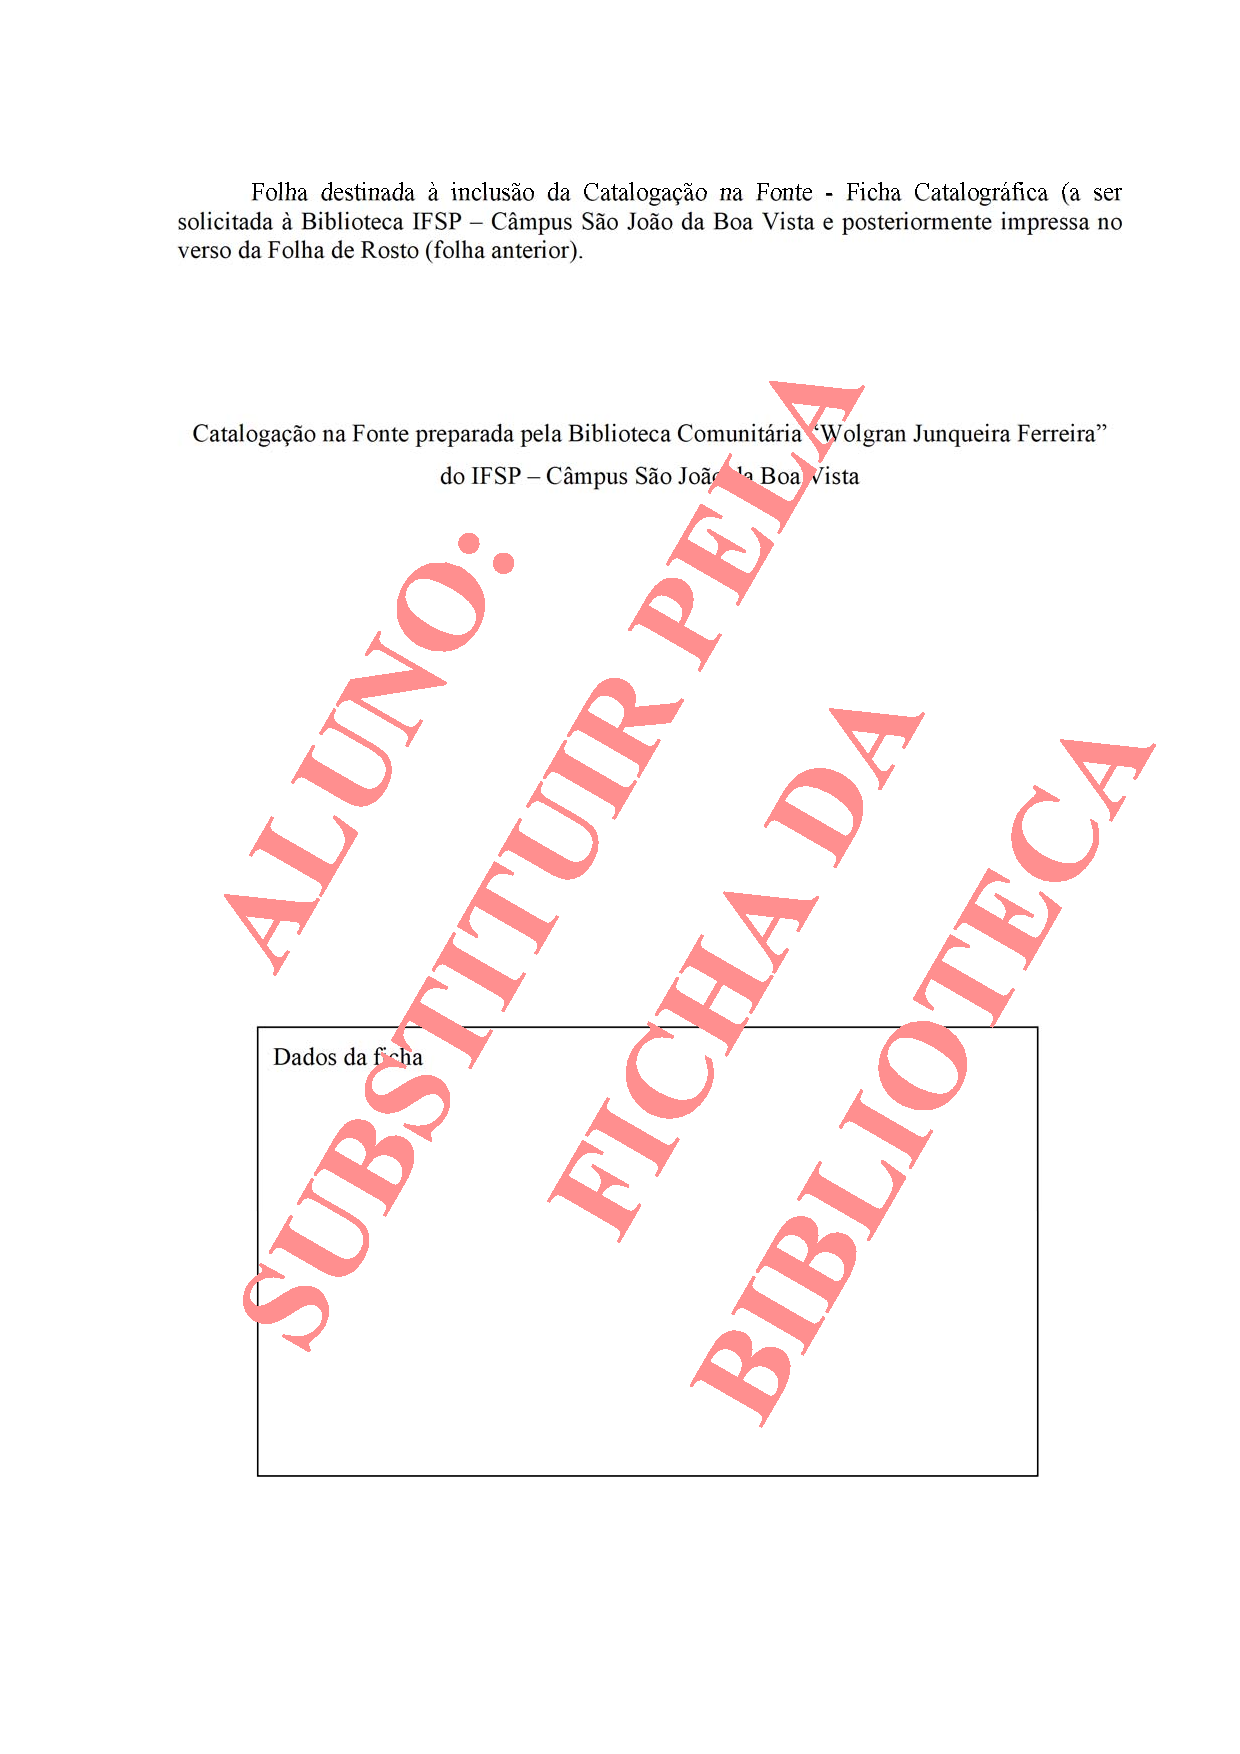
\includepdf{fichaCatalografica/exemploFichaCatalografica.pdf}
\end{fichacatalografica}

% ---
% Inserir folha de aprovação
% ---
%
% Este é um exemplo de folha de aprovação.
%
% A folha de aprovação final será inserida pelo Coordenador do Curso.
%

\begin{folhadeaprovacao}
	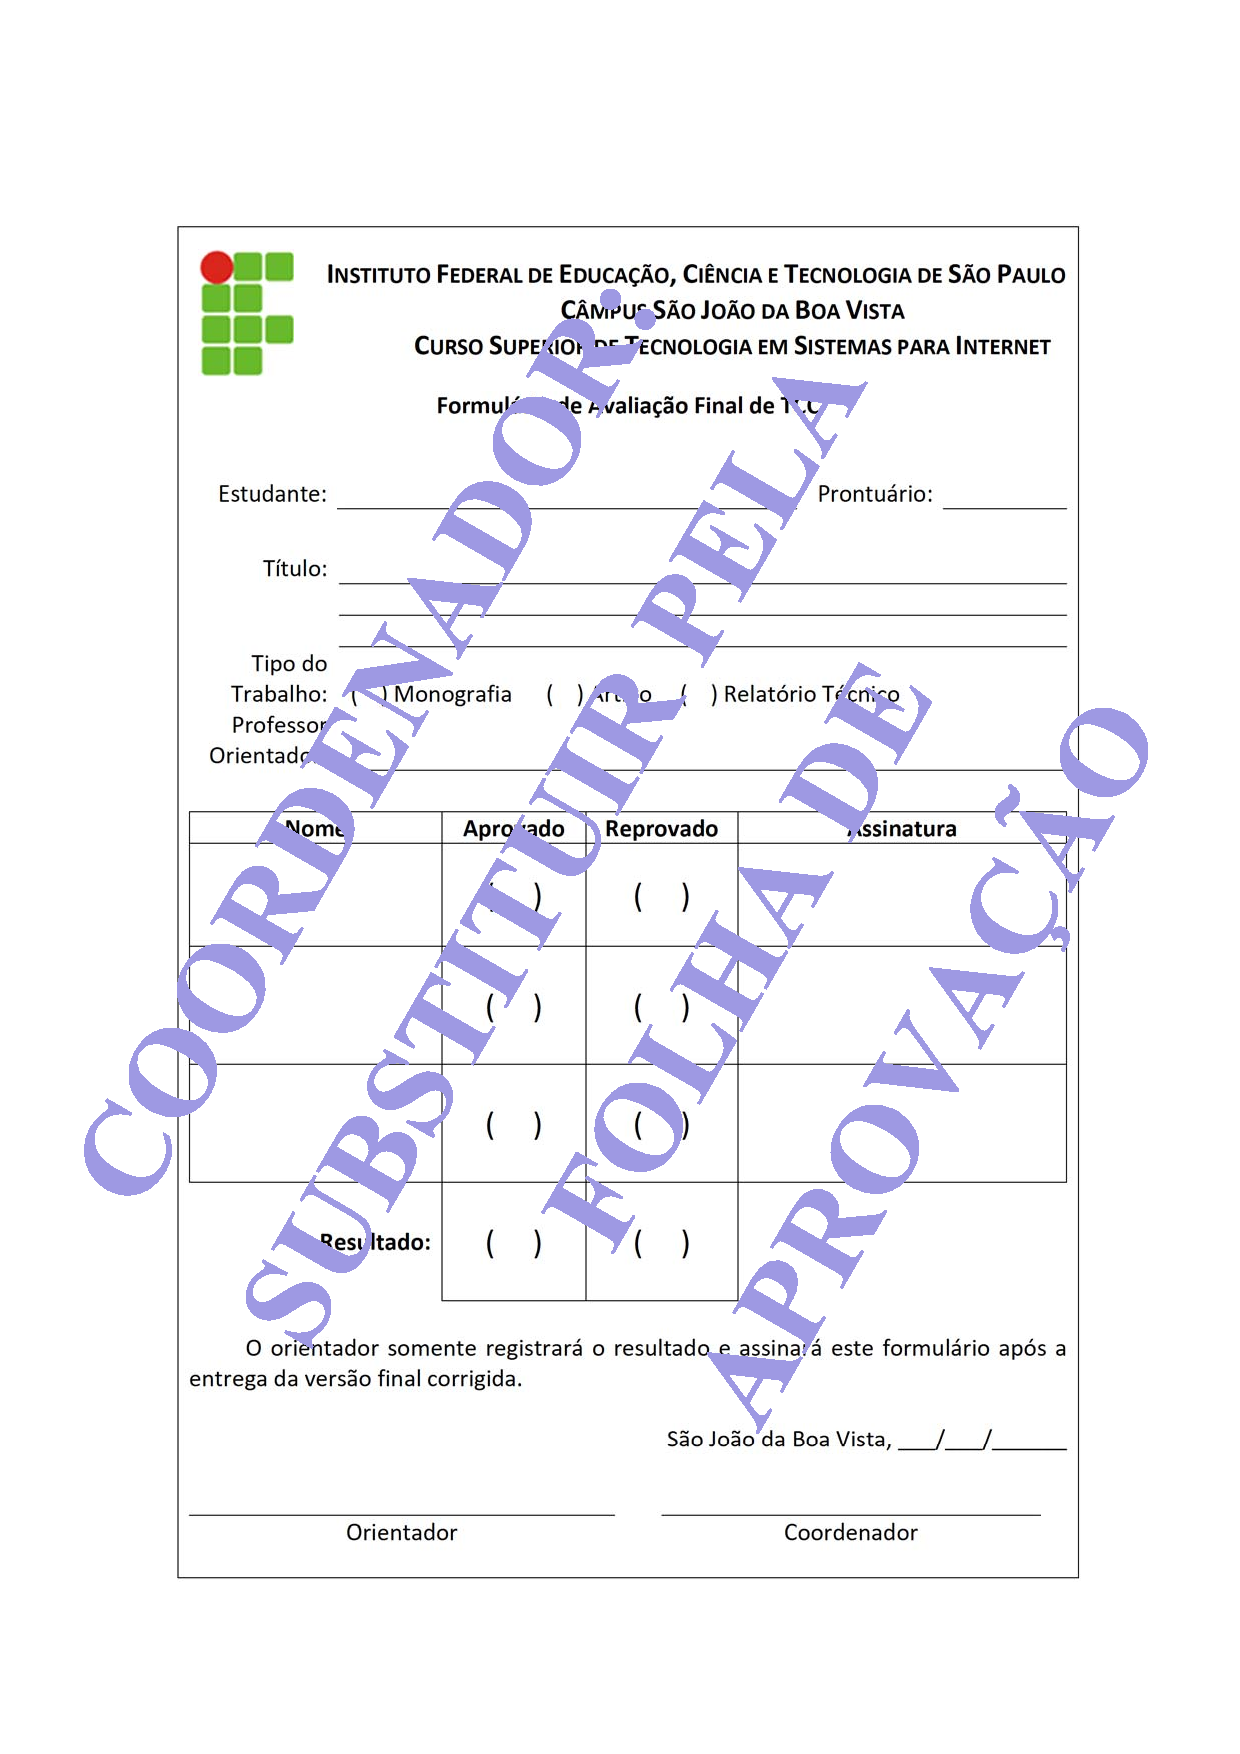
\includepdf{folhaAprovacao/exemploFolhaAprovacao.pdf}
\end{folhadeaprovacao}

% ---
% Dedicatória
% ---
\begin{dedicatoria}
	\vspace*{\fill}
	\centering
	\noindent
	\textit{Dedico este trabalho a minha mãe Sandra por toda paciência,  compreensão, carinho, amor, sacrifícios e esforços realizados para que esse momento se tornasse possível}
    \vspace*{\fill}
\end{dedicatoria}

% ---
% Agradecimentos
% ---
\begin{agradecimentos}
	Primeiramente a Deus, por estar comigo em todos os momentos.
	A minha irmã Eloá e minha companheira Bianca pelo companheirismo e paciência.
	Aos meus colegas, professores e coordenadores de graduação e pós-graduação.
	Cada um de vocês teve um papel importante em meu desenvolvimento pessoal e profissional.	
\end{agradecimentos}

% ---
% Epígrafe
% ---
\begin{epigrafe}
	
	\vspace*{\fill}
	\begin{comment}
	Epígrafe (Opcional). Pensamentos retirados de um livro, uma música, um poema, normalmente relacionado ao tema do trabalho, seguida de indicação de autoria. As epígrafes podem ser colocadas também nas folhas de abertura de cada capítulo
	\end{comment}.  
    
	\epigraph{``\emph{... se você passar muito tempo pensando, você nunca irá fazer nada.}''}{Bruce Lee}
	
\end{epigrafe}

% ---
% Resumos
% ---
\setlength{\absparsep}{18pt} % ajusta o espaçamento dos parágrafos do resumo
\begin{resumo}
	
	%Elemento obrigatório, constituído de uma sequência de frases concisas e objetivas, fornecendo uma visão rápida e clara do conteúdo do estudo. O texto deverá conter entre 150 a 250 palavras e ser antecedido pela referência do estudo. Também, não deve conter citações e deverá ressaltar o objetivo, o método, os resultados e as conclusões. O resumo deve ser redigido em parágrafo único, seguido das palavras representativas do conteúdo do estudo, isto é, palavras-chave, em número de três a cinco, separadas entre si por ponto e finalizadas também por ponto. Usar o verbo na terceira pessoa do singular, com linguagem impessoal (pronome SE), bem como fazer uso, preferencialmente, da voz ativa.
	
	%Uma abordagem prática sobre o Kotlin, a nova linguagem de programação oficial para desenvolvimento de novos aplicativos e manutenção de aplicações legadas para a plataforma Android, abordando as suas principais características e especificidades como: tipos de tipagem, estilo de syntaxe, motivo pelo qual foi criada, sua aplicabilidade ao dia-a-dia, compatibilidade com tecnologias e técnicas já existentes e consagradas no mercado de software, estrutura arquitetural e usabilidade em ambientes de desenvolvimento integrado como IntelliJ, Netbeans, Eclipse e Android Studio e editores de texto como Visual Studio Code. Isso será possível por meio da conversão de códigos originalmente desenvolvidos em Java (uma das linguagens influenciadoras) para o Kotlin tanto de forma manual como por recursos oferecidos pelos ambientes utilizados. %(FALTAM 30 PALAVRAS)
	
	%Estudo quali-quantitativo entre as linguagens de desenvolvimento de \textit{software} \textit{Java} e \textit{Kotlin}, com ênfase nos algoritmos utilizados na criação de aplicações móveis para os usuários da plataforma móvel \textit{Android}, com o objetivo de efetuar a constatação de qual tecnologia necessita de menores quantidades de caracteres, linhas de codificação e tamanho em \textit{bytes}, por meio de experimentos específicos como programas de Olá Mundo!, classes, operações matemáticas e por fim a elaboração de uma aplicação que efetua a conversão de medidas termométricas, implementado nas linguagens analisadas, apoiando-se no padrão de projeto Adapter. Com base nos recursos 
	%utilizando-se para tal, a plataforma Android Studio e seus recursos oferecidos como formatação e endentação.
	
	A evolução dos dispositivos móveis afeta não somente os seus usuários comuns, mas também todos os profissionais do ramo de tecnologia, por traz de toda a arquitetura de uma aplicação, seja ela simples ou \textit{rocket science}. A escolha da linguagem de programação deve levar em consideração inúmeros fatores, desde conhecimento e experiência do(s) envolvido(s), até as peculiaridades referentes ao ecossistema no qual almeja-se atingir. O presente trabalho de conclusão de curso, tem o objetivo de apresentar um estudo quali-quantitativo entre as linguagens de desenvolvimento de \textit{software} \textit{Java} e \textit{Kotlin}, com ênfase nos algoritmos utilizados na criação de aplicações móveis para os usuários da plataforma móvel \textit{Android}, com o objetivo de efetuar a constatação de qual tecnologia necessita de menores quantidades de caracteres, linhas de codificação e tamanho em \textit{bytes}, por meio de experimentos específicos como programas de Olá Mundo!, classes, operações matemáticas e por fim a elaboração de uma aplicação que efetua a conversão de medidas termométricas, implementado nas linguagens analisadas, apoiando-se no padrão de projeto Adapter. Dados os experimentos utilizados, obteve-se o resultado de que por meio da linguagem Kotlin, torna-se possível chegar aos mesmos resultados com Java, porém com a menor necessidade códigos clichês e desnecessários.
	
	\vspace{\onelineskip}
	
	\textbf{Palavras-chave}: Kotlin. Java. Desenvolvimento. Tecnologia.
	
\end{resumo}
\setlength{\absparsep}{18pt} % ajusta o espaçamento dos parágrafos do resumo
\begin{resumo}[Abstract]
	
	\begin{otherlanguage*}{english}
		
		%Elemento obrigatório. É a versão do resumo em português para o idioma de divulgação internacional. Deve ser antecedido pela referência do estudo.
		
		
The evolution of mobile devices affects not only its ordinary users, but also all professionals in the field of technology, behind all the architecture of an application, be it simple or rocket science. The choice of the programming language should take into account innumerable factors, from the knowledge and experience of the involved ones, to the peculiarities regarding the ecosystem in which one aims to attain. The aim of this work is to present a qualitative and quantitative study of Java and Kotlin software development languages, with emphasis on the algorithms used in the creation of mobile applications for users of the Android mobile platform, with the objective to make the verification of which technology needs smaller amounts of characters, coding lines and size in bytes, through specific experiments like Hello World !, classes, mathematical operations and finally the elaboration of an application that makes the conversion of thermometric measurements, implemented in the languages analyzed, based on the Adapter design pattern. Given the experiments used, we obtained the result that through the Kotlin language, it is possible to reach the same results with Java, but with the least need unnecessary codes.
		
		\vspace{\onelineskip}
		 
		\textbf{Keywords}: Kotlin. Java. Development. Technology.
		
	\end{otherlanguage*}

\end{resumo} 

% ---
% inserir lista de ilustrações
% ---
\pdfbookmark[0]{\listfigurename}{lof}
\listoffigures*
\cleardoublepage
% ---

% ---
% inserir lista de quadros
% ---
% \pdfbookmark[0]{\listofquadrosname}{loq}
% \listofquadros*
% \cleardoublepage
% ---

% ---
% inserir lista de tabelas
% ---
\pdfbookmark[0]{\listtablename}{lot}
\listoftables*
\cleardoublepage
% ---

% ---
% inserir lista de abreviaturas e siglas
% ---
\begin{siglas}
	\item[TDD] Test Driven Development (Desenvolvimento Orientado por Testes)
	\item[I/O] Input/Output (Entrada/Saída)
	\item[iOS] iPhone OS (Sistema operacional móvel da Apple)
	\item[HTML] Hypertext Markup Language (Linguagem de Marcação de Hipertexto)
	\item[CSS] Cascading Style Sheets (Folhas de Estilo em Cascata)
	\item[WWW] World Wide Web (Rede Mundial de Computadores)
	\item[GPS] Global Localization System (Sistema de Posicionamento Global)
	\item[XML] Extensible Markup Language (Linguagem de Marcação Extensível)
	\item[UML] Unified Modeling Language (Linguagem de Modelagem Unificada)
	\item[CRUD] Acrônimo para create, read, update e delete
	\item[macOS] Machintosh OS (Sistema operacional desktop da Apple)
\end{siglas}
% ---

% ---
% inserir lista de símbolos
% ---
% %\begin{simbolos}
%\	\item[$\alpha$] Letra grega minúscula Alfa
%\	\item[$\beta$] Letra grega minúscula Beta
%\\end{simbolos}
% ---

% ---
% inserir o sumário
% ---
\pdfbookmark[0]{\contentsname}{toc}
\tableofcontents*
\cleardoublepage
% ---






% ---------------------------------------------------------------------------------
%                                  ELEMENTOS TEXTUAIS
% ---------------------------------------------------------------------------------
\textual

\chapter{Introdução}
\label{cap:01}
%Neste capítulo será apresentada uma visão geral desse trabalho de conclusão de curso, com foco no contexto, justificativa e objetivos do presente trabalho.
%O objetivo deste documento é esclarecer aos autores o formato que deve ser utilizado nas monografias de TCC a serem submetidos ao final dos cursos de Graduação e Pós-Graduação do IFSP câmpus São João da Boa Vista.
%Neste documento estão listadas as seções obrigatórias que você deverá fornecer, bem como os exemplos dos comandos mais comuns que serão utilizados na construção de seu documento. Para pesquisar sobre mais comandos, recomenda-se a utilização do site \url{https://ctan.org/}, que é a biblioteca principal do \LaTeX, e o do site \url{https://tex.stackexchange.com} que é uma das principais comunidades para solução de dúvidas relacionadas a \LaTeX. Ambas são em inglês.
%Parte inicial do texto, na qual devem constar o tema e a delimitação do assunto tratado, objetivos da pesquisa e outros elementos necessários para situar o tema do trabalho, tais como: justificativa, procedimentos metodológicos e estrutura do trabalho, tratados de forma sucinta. Salienta-se que os procedimentos metodológicos e o embasamento teórico são tratados, posteriormente, em capítulos próprios e com a profundidade necessária ao trabalho de pesquisa.
 %\section {Contextualização}
 Em relação ao desenvolvimento de \textit{software} voltado para dispositivos móveis, existem inúmeras opções de tecnologias. Para criar aplicativos nativos voltados para usuários da plataforma \textit{Android}, pode-se utilizar a linguagem \textit{Java} por meio do Ambiente de Desenvolvimento Integrado (\textit{Integrated Development Environment - IDE}) \textit{Android Studio}. Já para o desenvolvimento nativo voltado para usuários de \textit{iOS}, pode-se optar pela linguagem \textit{Swift} ou \textit{Objective-C} por meio da \textit{IDE} \textit{Xcode}. Para criar aplicações híbridas (\textit{Android} e \textit{iOS}) existem mais opções, como o \newcommand{\Csh}{\textit{C}{\lserif\#}}\Csh{} e o \textit{.NET Framework} por meio do plugin \textit{Xamarin} disponível na \textit{IDE} \textit{Visual Studio}, ou o \textit{Ionic Framework} utilizando \textit{HTML}, \textit{CSS}, \textit{Node.js}, \textit{TypeScript} e \textit{Apache Cordova} utilizando as \textit{IDE's} \textit{Android Studio} e \textit{Xcode}. Cada tecnologia citada anteriormente possui suas especificidades como ecossistema próprio, sintaxe, nomes, tipagem, semântica, um ou mais paradigmas de programação e curva de aprendizado. Com a variedade de opções, pode ser difícil escolher a ideal para cada situação/contexto.

 \citeauthorandyear{TuckerNoonan2009} disseram que, \begin{citacao}Talvez a maior motivação para o desenvolvimento de linguagens de programação nas últimas décadas tenha sido a rápida evolução da demanda de poder computacional e as novas aplicações por parte de uma grande e diversa comunidade de usuários. \end{citacao}
 
 Segundo \citeauthorandyear{Fowler2009}, "Qualquer tolo consegue escrever código que um computador entenda. Bons programadores escrevem código que humanos possam entender". Independente da tecnologia, o propósito sempre é solucionar um problema e/ou atender uma necessidade específica.
 %Como as linguagens adotam os padrões de lógica de programação (variáveis, comentários, identificadores e atribuições, operações aritméticas, lógicas, repetição e vetores)
 %é necessário possuir algum domínio da linguagem e ambiente de desenvolvimento escolhidos.¨
 Porém, apenas escrever algoritmos
 não é o suficiente, códigos não endentados, variáveis e operações com nomenclaturas pouco intuitivas, excesso ou falta de comentários e operações muito extensas e com várias responsabilidades podem ocasionar na dificuldade de manutenção e falta de flexibilidade.
 
 \citeauthorandyear{Martin2009} cita que, \begin{citacao}"[...] A lógica deve ser direta para dificultar o encobrimento de \textit{bugs}\footnote{Defeito, falha ou erro no código de um programa que provoca seu mau funcionamento.}, as dependências mínimas para facilitar a manutenção, o tratamento de erro completo de acordo com uma estratégia clara e o desempenho próximo do mais eficiente de modo a não incitar as pessoas a tornarem o código confuso com otimizações sorrateiras. O código limpo faz bem apenas uma coisa. \end{citacao}
 
 Linguagens de programação mais verbosas como por exemplo o \textit{Java}, precisam de mais palavras e/ou palavras mais longas e mais símbolos que o necessário para expressar adequadamente a intenção do código, o que não é necessariamente um problema, mas sim a característica da linguagem. Uma tentativa de diminuir a verbosidade tão comum da linguagem \textit{Java} removendo códigos desnecessários para obter algoritmos mais concisos e sucintos foi a criação da biblioteca \textit{Project Lombok}. \citeauthorandyear{Josh2019} diz que, "A biblioteca substitui o \textbf{código clichê} por anotações fáceis de usar, [...] tornando o código mais fácil de ler e menos sujeito a erros e tornando os desenvolvedores mais produtivos"\footnote{De acordo com \citeonline{Josh2019}, \textit{Project Lombok is a mature library that reduces boilerplate code. The library replaces boilerplate code with easy-to-use annotations[...] making code easier to read and less error-prone and making developers more productive}.}, porém como não houve nenhuma modificação na linguagem, código clichê pode acabar resultando em \textbf{mau cheiro de código} (\textit{code smell}). Segundo \citeauthorandyear{Turini2014}, “Mau cheiro é o termo utilizado quando um determinado código possui algum indício de que está precisando ser \textbf{refatorado}".

De acordo com \citeauthorandyear{Fowler2009}, "[...] o propósito da refatoração é tornar o \textit{software} mais fácil de entender e modificar". Em 1997 foi criada uma metodologia ágil denominada de Programação Extrema (\textit{Extreme Programming} - XP), com intuito de facilitar o desenvolvimento de \textit{software} e aprimorar a qualidade dos projetos, sendo a refatoração de código, umas das principais práticas utilizadas.
Em 1999 foi criado o Desenvolvimento Orientado a Testes (\textit{Test Driven Development} - TDD), onde na primeira etapa se escreve o teste para uma funcionalidade ainda inexistente, na segunda etapa se escreve a funcionalidade a ser testada e na terceira e última o código é refatorado, diminuindo assim futuros \textit{bugs}. Segundo \citeauthorandyear{Guerra2014}, o TDD "é uma técnica de desenvolvimento e projeto de \textit{software} na qual os testes são criados antes do código de produção. É uma técnica que vem se tornando cada vez mais popular no mercado e mais atenção da academia".

Conforme \citeauthorandyear{Martin2009}, "Não basta escrever um código bom. Ele precisa ser mantido sempre limpo". Devido à grande variedade de linguagens, tecnologias, metodologias de desenvolvimento disponíveis no mercado, até mesmo falta de tempo, escolher a linguagem de programação ideal para resolução de um determinado problema e escrever um código limpo independente do paradigma pode ser uma tarefa árdua para desenvolvedores de todos os níveis.

 %Durante o \textit{Google} I/O 17, que é uma conferência anual voltada para o desenvolvimento de aplicações para os seus próprios sistemas operacionais, mais especificamente o \textit{Android}, a linguagem \textit{Kotlin} entrou para o seleto grupo de linguagens oficiais de desenvolvimento de aplicativos para a plataforma da \textit{Google}. Isso já era esperado, pois \textit{Kotlin} vinha recebendo muitos feedbacks positivos da comunidade de desenvolvedores \cite{Resende2018}. Já estavam presentes nesse seleto grupo as amplamente consagradas linguagens \textit{Java} e C++.  

%Criada em 2011 pela JetBrains, criadora de ambientes de desenvolvimento integrado, IDE na sigla em Inglês, e outras ferramentas direcionadas para desenvolvedores de \textit{software} e gestores de projeto, a linguagem recebeu o nome de uma ilha localizada na Rússia, onde a equipe criadora da linguagem residia. O objeto era suprir deficiências encontradas em outras linguagens. Em fevereiro de 2016, foi lançada a versão 1.0 estável do \textit{Kotlin}, sob licença Apache de código aberto. A ideia era criar uma nova linguagem estaticamente tipada para a JVM \cite{Resende2018}.

%Por ser compatível com o Kit de Desenvolvimento \textit{Java} (JDK na sigla em Inglês) versão 6, possibilita que programas criados em \textit{Kotlin}, sejam compatíveis com qualquer versão do \textit{Android}. Um arquivo \textit{Kotlin} possui extensão .kt, o compilador do \textit{Kotlin} transcreve esse arquivo .kt para .class (bytecode do \textit{Java}), com isso, funciona em todos os dispositivos que suportam a linguagem \textit{Java}. A linguagem da JetBrains suporta os paradigmas de programação orientada a objetos e funcional, além de ser totalmente suportada pela IDE oficial de desenvolvimento \textit{Android}, que no momento em que esse artigo fio escrito é plataforma \textit{Android} Studio. 

 %\cite{Lecheta2018} diz que a linguagem \textit{Kotlin} possui uma síntaxe simples interoperabilidade total com \textit{Java}. Portanto, o \textit{Kotlin} não vem para substituir nenhuma das linguagens e/ou tecnologias presentes e consagradas no mercado de desenvolvimento de \textit{software}, mas sim para oferecer mais uma opção para os desenvolvedores no momento da criação de novas aplicações móveis e atualização de aplicações legadas, uma vez que tudo que já foi desenvolvido em todas as bibliotecas do Android "conversam” com \textit{Kotlin}, sem precisarem ser reescritas. 

%Nos dois capítulos posteriores serão apresentadas de maneira resumida visões gerais sobre a história da linguagem \textit{Java} e da tecnologia \textit{Android} respectivamente, para que seja possível, no capítulo seguinte entrar de vez na linguagem que vem despertando cada vez mais curiosidade no mundo do desenvolvimento de \textit{software}.

\section{Justificativa}

 Durante o \textit{Google} I/O 17, uma conferência anual voltada para o desenvolvimento de aplicações para os seus próprios sistemas operacionais, mais especificamente o \textit{Android}, a linguagem \textbf{\textit{Kotlin}} entrou para o seleto grupo de linguagens oficiais de desenvolvimento de aplicativos para a plataforma da \textit{Google}.  \citeauthorandyear{Resende2018} diz que, "isso já era esperado, pois \textit{Kotlin} vinha recebendo muitos \textit{feedbacks} positivos da comunidade de desenvolvedores".

A linguagem \textit{Kotlin} possui uma sintaxe simples, pouco verbosa e concisa. Segundo \citeauthorandyear{Lecheta2018}, "uma das grandes vantagens do \textit{Kotlin} é a sintaxe moderna e expressiva, pois, se comparado ao \textit{Java}, pode-se escrever o mesmo código com muito menos linhas".

O propósito deste trabalho é elucidar de forma comparativa e concisa as vantagens de se optar pela linguagem de programação \textit{Kotlin}, em meio às múltiplas alternativas. Aproveitando os recursos atuais e expressivos da linguagem para desenvolver um código menos clichê, otimizando assim o processo de manutenção e de teste. 

%De acordo com o site oficial da linguagem, disponível em \url{https://www.jetbrains.com/}, atualmente grandes empresas como \textit{Pinterest, Uber, Coursera, Atlassian} e \textit{Evernote}, entre outras, estão utilizando a linguagem da JetBrains de alguma forma no dia-a-dia de suas corporações.

%O webiste Stack Overflow referência para o mundo dos desenvolvedores, mantido pela empresa Stack Exchange, realizou uma pesquisa com mais de 100.000 usuários de sua plataforma em 2018.\cite{StackOverFlow2018} Podem-se destacar os seguintes resultados a respeito da linguagem \textit{Kotlin}:
 %\begin{itemize}
 %  \item {2ª} linguagem de programação mais amada;
 %  \item {4ª} linguagem de programação mais procurada;
%   \item {22ª} tecnologia mais popular.
 %\end{itemize}
 
%https://insights.stackoverflow.com/survey/2018/#technology
%De acordo com \cite{Tiobe2018} que é uma lista ordenada de linguagens de programação, classificada pela freqüência de pesquisa na web usando o nome da linguagem como a palavra-chave, divulgou em seu site, o seguinte resultado:
 %\begin{itemize} 
 %\item A linguagem \textit{Kotlin} subiu de {39ª} para a {31ª} colocação %como linguagem de programação mais utilizada em janeiro de %2019.
 %\end{itemize}
  %https://www.tiobe.com/tiobe-index/

%Com os dados apresentados a cima, pode-se chegar a conclusão de que a linguagem ganha cada vez mais espaço, e sua adoção está cada vez mais comum entre empresas e desenvolvedores de \textit{software}. \textit{Kotlin} entrará no top 20. Vemos uma adoção rápida no mercado de aplicativos móveis industriais dessa linguagem. \cite{Tiobe2018}.

%https://www.tiobe.com/tiobe-index/

\section{Objetivos}
Nesta secção serão apresentados os objetivos gerais e específicos desta pesquisa.

\subsection{Objetivo Geral}

%Esta pesquisa tem o objetivo de demonstrar como utilizar linguagem de programação \textit{Kotlin} para escrever códigos diretos, de forma mais rápida, menos verbosos e de fácil interpretaçã. Resultando em código limpo para que seja fácil de refatorá-lo frente a novas necessidades.
O objetivo dessa pesquisa é apresentar uma análise quali-quantitativa sobre a utilização da linguagem de programação \textit{Kotlin}, referente às questões de usabilidade em desenvolvimento de \textit{software} com foco em aplicações móveis.%, comparando com outras linguagens de programação existentes no mercado.

%Kotlin possui uma sintaxe simples, pouco verbosa e concisa, o que faz com que códigos escrit

\subsection{Objetivos Específicos}

Os passos abaixo descrevem as etapas necessárias para a conclusão do objetivo geral da pesquisa:

\begin{itemize}
	\item Estudar a linguagem de programação \textit{Kotlin} e questões relacionadas com a usabilidade na programação;
	\item Definir métricas de usabilidade na programação;
	\item Comparar o uso do \textit{Kotlin} em relação a linguagem de programação \textit{Java};
	\item Analisar quanti-qualitativamente o uso do \textit{Kotlin}, evidenciando as métricas de usabilidade estabelecidas.
\end{itemize}

\section{Organização deste Trabalho}

O presente trabalho está estruturado em cinco capítulos. No primeiro capítulo é apresentada uma breve introdução, objetivos buscados e justificativa da pesquisa. No segundo capítulo são expostos os textos referenciais. A metodologia do projeto é demonstrada no terceiro capítulo. No quarto capítulo são exibidos os resultados finais. As conclusões são desenvolvidas no quinto capítulo.
\chapter{Revisão da Literatura}
\label{cap:02}
Neste capítulo, serão apontados os levantamentos bibliográficos realizados para esta pesquisa. Nele, serão apresentados os seguintes temas: dificuldades existentes na programação, linguagens de programação nativas e híbridas voltadas para desenvolvimento de dispositivos móveis, qualidade de código e trabalhos relacionados a este trabalho.

\section{Dificuldades Existentes na Programação}

Devido a rápida popularização dos aplicativos e sua fácil e prática utilização, os iniciantes podem acabar optando por entrar no ramo de desenvolvimento de \textit{software} com a ideia de conquistar uma vida financeira próspera por meio da disponibilização de uma aplicação simples em qualquer uma das famosas lojas disponíveis, e isso sem maiores esforços. No entanto, o aprendizado em tecnologia da informação, assim como em qualquer outra área/ramo, demanda empenho e prática. Um estudante de ciências contábeis, administração leva um tempo para se adaptar à normas e cálculos atuais, da mesma forma como um estudante da área da saúde não realiza manobras de salvamento sem conhecimento prévio, o mesmo conceito se aplica na programação.
Pular os fundamentos da área pode ser uma das piores práticas, pois o conhecimento básico aplica-se a todos os tipos de desenvolvimento, seja ele voltado para \textit{web}, \textit{desktop} ou \textit{mobile} \cite{Unipe2018}. 

O ato de desenvolver uma simples solução ou um \textit{software} extremamente complexo demanda muito mais do que apenas escrever um algoritmo em uma determinada linguagem e tecnologia.
O mais comum na área de tecnologia, é trabalhar e dar manutenção em um sistema que já está sendo utilizado, e que foi escrito por outros profissionais, para realizar qualquer modificação, faz-se necessário \textbf{compreender} toda a estrutura, conseguir visualizar/imaginar as consequências de cada futura alteração. Na maioria das vezes um código mais enxuto é sempre superior a outro com inúmeros trechos inúteis de códigos desnecessários. Nesse momento fazem-se úteis as melhorias internas como \textbf{reescrita} usando técnicas como \textit{TDD}, programação em par, revisão de código e versionamento de projeto \cite{Gabs2018EscreverCodigo}.

O mercado de tecnologia da informação é um dos poucos onde a demanda por profissionais qualificados de todos os níveis cresce independente de qualquer fator interno ou externo. Porém, a escolha de tecnologias para estudar, aplicar em um projeto ou solucionar problemas é imensa, principalmente para os ingressantes, essa busca pode ser um tanto quanto custosa. O primeiro passo para a escolha da linguagem adequada deve ser a definição do mercado de atuação \cite{Scudero2017}.

Anualmente são divulgados índices ranqueados sobre as linguagens, mesmo assim as opções são inúmeras. 
Para não errar na escolha, deve-se optar entre as tecnologias de \textit{front-end} (que estão em pleno crescimento) como \textit{HTML}, \textit{CSS}, \textit{JavaScript} e \textit{frameworks JavaScript} ou linguagens \textit{back-end} (maior empregabilidade), dentre as principais estão \textit{Java}, \textit{C\#}, \textit{Python} e \textit{Swift}.
A iniciação no mundo de desenvolvimento de \textit{software} com \textit{JavaScript}, que aplica-se tanto em aplicações \textit{front-end} como no \textit{back-end} tende a ser mais indicado para os iniciantes, pois necessita-se apenas de um navegador de internet que todos já têm/tiveram contato, e um editor de texto, o que é quase nada se comparado a instalação e configuração de um ambiente de desenvolvimento integrado e de um conjunto de desenvolvimento de \textit{software} \cite{Scudero2017}. Essa facilidade no início levou o \textit{JavaScript} a ser introduzido em renomadas instituições de ensino estadunidenses, substituindo assim, o lugar do \textit{Java} como linguagem introdutória para muitos alunos e turmas. Tanto \textit{C\#} como o \textit{Java} possuem uma curva de aprendizado maior, o que acaba tornando-se pouco atrativo para novatos, mas que em contrapartida possuem comunidades fortes e grandes companhias dando suporte, o que eleva o índice de oferta, procura e contratação \cite{Scudero2017}. 

\subsection{Metodologias Ágeis}
%cap 1 pag 4 +/-
Em sua maior parte, todas as técnicas ágeis empregam e recomendam o desenvolvimento dividido/subdividido em pequenas etapas, e estas etapas tendem a ser pouco extensas, o que por sua vez, assegura o parecer contínuo e resultados mais velozes mediante possíveis alterações, tendo em vista substituir técnicas mais antigas e ineficazes, porém ainda utilizadas como a metodologia de desenvolvimento em cascata, conforme Figura 1. \cite{gomes2014agile}.

\FloatBarrier
\begin{figure*}[!htbp]
	\centering
		\caption{Metodologia \textit{Waterfall} (Cascata)} 
	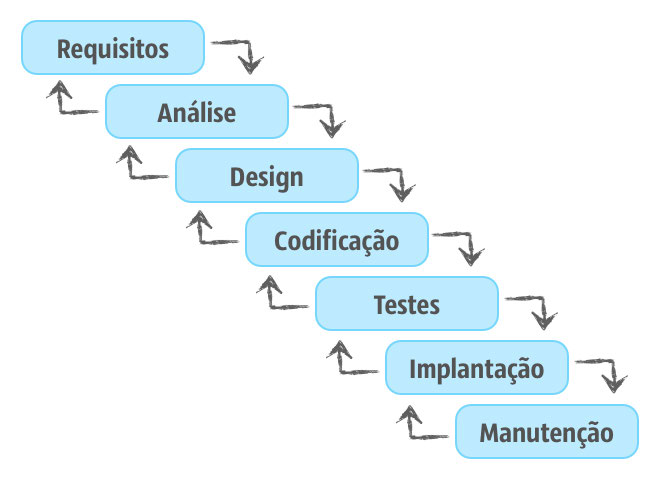
\includegraphics[scale=0.4]{imagens/CASCATA}
	\subcaption{\textbf{Fonte:} \cite{gomes2014agile}}
	\label{fig:figura1}
\end{figure*}
\FloatBarrier

Dentre as inúmeras técnicas denominadas ágeis presentes e disponíveis no mercado, pode-se destacar:

\begin{itemize}
%cap 1 pag 12 +/-
\item{\textbf{\textit{Scrum}}}: Desenvolvido em meados de 1990 por Ken Schwaber, Jeff Shuterlande Mike Beedle, o \textit{framework Scrum} está entre os mais aplicadas no mercado, com ênfase na administração de projetos, a ferramenta fomenta a acabativa\footnote{Neologismo criado por Stephen Kanitz, que segundo o autor é "a capacidade que algumas pessoas possuem de terminar aquilo que iniciaram ou concluir o que outros começaram \cite{Acabativa}."} no desenvolvimento de \textit{software} e na maioria dos casos é implementado juntamente com outras ferramentas ágeis \cite{wildt2015extreme}. 
%cap 1 pag 12 +/-
\item{\textbf{\textit{eXtreme Programming}}}: Criado por Kent Beck, Ward Cunningham e Ron Jeffries, comumente chamado de \textit{XP}, a técnica \textit{eXtreme Programming} foi idealizada para equipes intermediárias, o \textit{XP} foca principalmente na programação e nos testes. Seu propósito é a elevação do nível de confiabilidade, manutenabilidade e reusabilidade dos algoritmos desenvolvidos \cite{wildt2015extreme}.

\item{\textbf{\textit{Kanban}}}:
Na língua japonesa \textit{Kanban} quer dizer cartão sinalizador. Em contrapartida das outras técnicas ágeis, o \textit{Kanban} não impõe etapas, a ferramenta visa o aumento de produtividade por meio de uma melhor apresentação do \textit{workflow}, separando as atividades em etapas. É a metodologia ágil que menos impõe regras \cite{gomes2014agile}.
\end{itemize}

Em Scrum, XP e Kanban, há uma menor quantidade de prescrições a se seguir, facilitando a adaptação, conforme Figura 2.

\FloatBarrier
\begin{figure*}[!htbp]
	\centering
		\caption{Métodos ágeis e seus níveis de prescrição e adaptação} 
	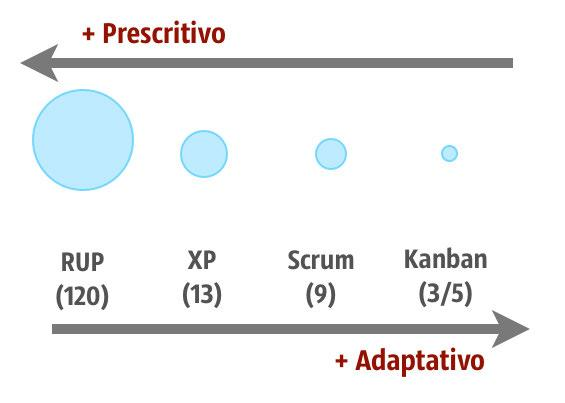
\includegraphics[scale=0.5]{imagens/prescricao}
	\subcaption{\textbf{Fonte:} \cite{gomes2014agile}} 
	\label{fig:figura2}
\end{figure*}
\FloatBarrier

\section{Tecnologias e Linguagens de Programação para Dispositivos Móveis}

Quando fala-se em aplicação móvel, na verdade referem-se aos programas que realizam operações específicas em \textit{smartphones}, \textit{tablets} e dispositivos \textit{wearables} \cite{Abranches2018}.

\subsection{Desenvolvimento Nativo para \textit{Android}}

Apesar das aplicações móveis multiplataforma ganharem mais espaço a cada ano, as aplicações mais bem-sucedidos do mercado mundial como o \textit{Facebook Messenger} e \textit{Whatsapp} foram desenvolvidos de forma nativa \cite{Abranches2018}. 

\subsubsection{Linguagem \textit{Java}}
%páginas 02 e 03%
A linguagem de programação \textit{Java} já a algum tempo é predominante na \textit{web} (\textit{World Wide Web} - WWW), a linguagem transformou a compreensão sobre desenvolvimento de sistemas, tornando-se indispensável para aqueles que almejam serem especialistas da área. Com fortes heranças de linguagens como \textit{C} e \textit{C++} e incorporando avanços e outras capacidades, \textit{Java} foi criado por James Gosling, Patrick Naughton, Chris Warth, Ed Frank e Mike Sheridan em 1991 na até então \textit{Sun Microsystems} atual \textit{Oracle Corporation}. Com o objetivo de se obter uma linguagem portátil, livre de outros programas e que fosse capaz de ser funcional nos aparelhos digitais comuns no dia-a-dia \cite{Herbert}.

%página 16 e 17
A linguagem ganhou grande repercussão em 1995 devido a sua mobilidade, possível graças a sua \textit{Java Virtual Machine} (Máquina Virtual \textit{Java} - \textbf{\textit{JVM}}) que atua como uma tradutora, transformando todo o código \textit{\textbf{bytecode} \textit{Java}} em um idioma compreendido pelo computador, independente se o sistema operacional utilizado é um \textit{Windows}, \textit{Linux} ou \textit{macOS}. Com a ausência de uma \textit{JVM}, seria necessário escrever códigos modificados para cada uma das plataformas \cite{Burd}, conforme apresentado na Figura 3.

\FloatBarrier
\begin{figure*}[!htbp]
	\centering
		\caption{Execução de um programa de computador}
	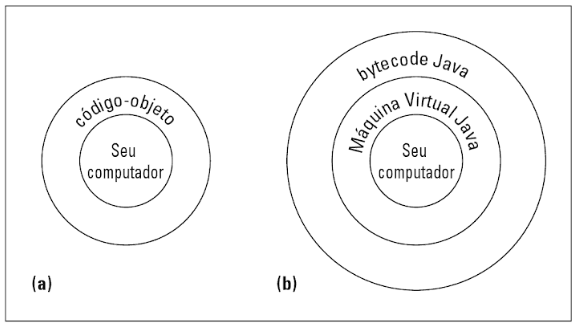
\includegraphics[scale=0.5]{imagens/JVM}
	\subcaption{\textbf{Fonte:} \citeauthorandyear{Burd}}
	\label{fig:figura3}
\end{figure*}
\FloatBarrier

\subsubsection{Plataforma \textit{Android}}

%pag 6
Criado pela \textit{Android Inc}, o sistema \textit{Android} foi comprado pela \textit{Google} em 2005, e desde 2007 vem sendo suportado pela \textit{OHA} (\textit{Open Handset Aliance}) grupo formado por gigantes da tecnologia como \textit{HTC}, \textit{Sony}, \textit{Dell}, \textit{Motorola}, \textit{Qualcomm}, \textit{Texas Instruments}, a própria \textit{Google}, \textit{Samsung}, \textit{LG}, \textit{T-mobile}, \textit{Sprint Corporation}, \textit{Nvidia}, \textit{Wind River Systems}, \textit{Asus}, \textit{Intel} e outras \cite{DeitelDeitelWald2016}.

%pag 4
Aplicativos móveis voltados para a plataforma portátil da \textit{Google}, devem ser criados com a linguagem de programação \textit{Java}, escolhida por ser uma das mais utilizadas pelos desenvolvedores, empresas e instituições de ensino e não ter nenhum custo, uma vez que é \textit{open source}\footnote{A expressão \textit{open source} de origem americana, remete a \textit{softwares} que possuem o seu código fonte aberto para contribuições. \cite{openSourceCanalTech}}  Com isso, desenvolvedores com anos, tendem a ter uma curva de aprendizado pequena em relação ao \textit{Android}, se comparado aos programadores que não possuem experiência com a linguagem \cite{DeitelDeitelWald2016}.

%pag 11
Aparelhos com o sistema operacional \textit{Android} possuem funcionalidades como acesso à internet, música, vídeo, Sistema de Posicionamento Global (\textit{Global Positioning System} - \textit{GPS}), câmera, tela sensível ao toque, dentre outras inúmeras funções. A \textit{Play Store} é a loja oficial para adicionar, avaliar, procurar e realizar o \textit{download} das aplicações disponíveis \cite{DeitelDeitel2016}.

O sistema operacional da \textit{Google} tem previsão de continuar como o mais vendido até 2022 \cite{IDC}. Conforme Tabela~\ref{tab:tabela1} e Figura 4.

\FloatBarrier
\begin{table}[!htbp]
\centering
\caption{Participação no mercado mundial de \textit{smartphones}.}
	\begin{tabular}{ c | c | c | c | c | c | c | c }
		\hline
		\textbf{Ano} & \textbf{2016} & \textbf{2017} & \textbf{2018} & \textbf{2019}  & \textbf{2020} & \textbf{2021} & \textbf{2022}  \\ \hline
		\textit{Android}      & 84,6\%        & 85,1\%        &  84,7\%       & 85,2\%         & 85,3\%        & 85,4\%        & 85,5\%  \\ \hline
		\textit{iOS}          & 14,7\%        & 14,7\%        & 15,1\%        & 14,8\%         &14,6\%         & 14,6\%        & 14,5\%     \\ \hline
		Outros       & 0,7\%         & 0,2\%         & 0,1\%         & 0,1\%          & 0,1\%         & 0,1\%         & 0,1\% \\ \hline
	\end{tabular}
	\\ \vspace{0.2cm}
		\subcaption{\textbf{Fonte:} Adaptado pelo autor - \cite{IDC}}
	\label{tab:tabela1}
\end{table}
\FloatBarrier

\FloatBarrier
\begin{figure*}[!htbp]
	\centering
		\caption{Gráfico de participação no mercado mundial de \textit{smartphones}.}
	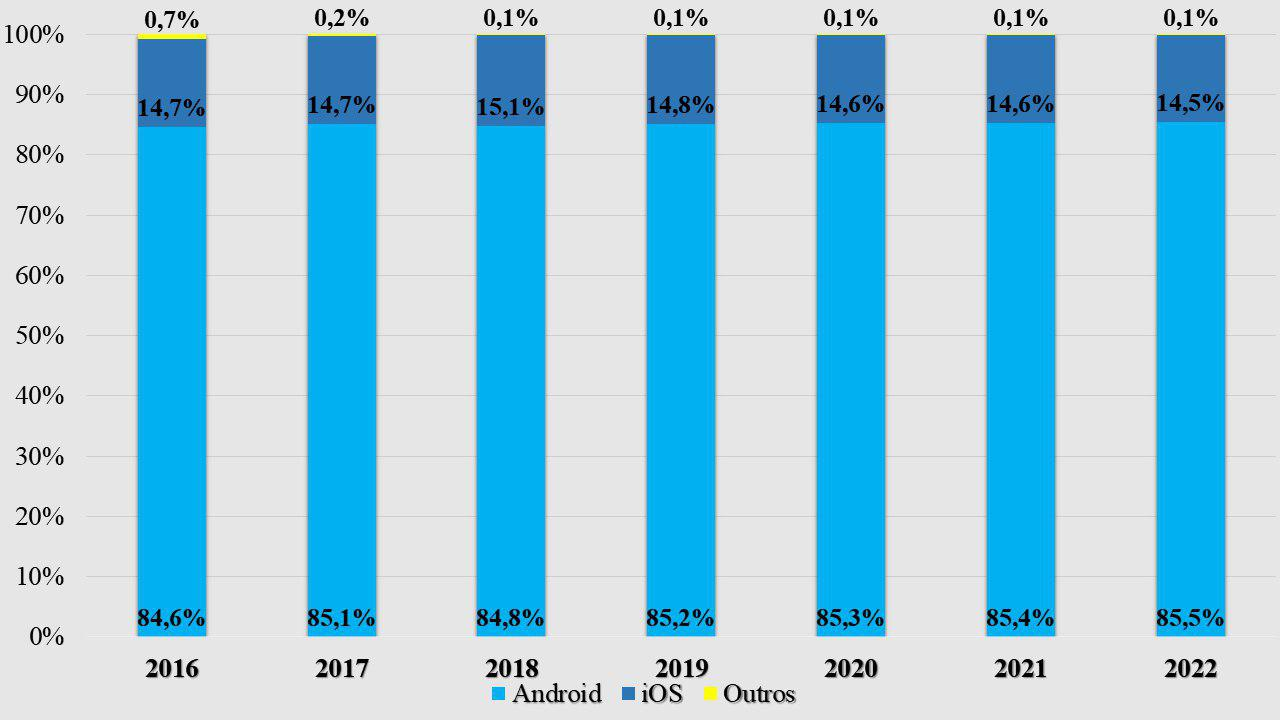
\includegraphics[scale=0.4]{imagens/IDC}
	\subcaption{\textbf{Fonte:} Adaptado pelo autor - \cite{IDC}}
	\label{fig:figura4}
\end{figure*}
\FloatBarrier

\subsection{Desenvolvimento Nativo para \textit{iOS}}

%pag 23
Tanto os usuários como os desenvolvedores que buscam por um \textit{design} mais sofisticado, uma riqueza maior em detalhes, aliados a uma comunicação diferenciada com o aparelho móvel, encontram como opção o \textit{iPhone}, que possui \textit{iOS}, o sistema operacional móvel da empresa americana \textit{Apple Inc.}, o mais utilizado após o \textit{Android} \cite{Lecheta2016_IOS_&_IPAD}.

%pags 23 e 24
Anunciado em 2007 em uma conferência voltada para programadores, no mesmo ano o \textit{smartphone iPhone} conseguiu ganhar seu lugar de destaque entre os usuários comuns e do mundo da tecnologia, devido a capacidade e qualidade dos recursos presentes no pequeno aparelho móvel, obteve também a atenção dos programadores, uma vez que sua loja oficial, a \textit{Apple Store} prometia uma gratificação, o que até o momento era novidade \cite{Lecheta2016_IOS_&_IPAD}.

%pags 2
Apesar de lançado em 2007, somente no ano seguinte tornou-se possível programar voltado para o \textit{iOS}, por meio do Kit de Desenvolvimento de \textit{Software} (\textit{Software Development Kit - SDK}), porém o \textit{SDK} passou a ser gratuito apenas três anos mais tarde. Para utilizar-se o \textit{iOS SDK}, é obrigatório possuir um computador com no mínimo o sistema operacional \textit{macOS X} instalado, caso contrário, não será possível nem mesmo realizar o \textit{download}. Recentemente, o \textit{SDK }passou a ser disponibilizado com o ambiente integrado oficial de desenvolvimento para a plataforma \textit{iOS}, o \textit{Xcode IDE} \cite{Steil_IOS}.

%pags 187 
\subsubsection{Linguagem \textit{Objective-C}}
Adquirida e licenciada em 1988 pela empresa \textit{Apple Inc.}, a linguagem 
\textit{Objective-C} foi fundamental no desenvolvimento de aplicações voltadas para \textit{iOS} e \textit{macOS}. Pode-se dizer que apesar da diferença na escrita de algoritmos, \textit{Objective-C} é na verdade \textit{C} com o acréscimo de várias funcionalidades como o paradigma de programação, portanto \textit{Objective-C} é totalmente interoperável com tudo que já existe e que foi escrito originalmente utilizando-se a linguagem \textit{C} \cite{Steil_IOS}.  

Dado ao avanço das linguagens de programação e das tecnologias envolvidas, o \textit{Objective-C} acabou tornando-se um tanto quanto obsoleto quando comparado a outras linguagens mais sucintas e com curva de aprendizado consideravelmente inferiores. Para mudar esse cenário, e fazer com o que a programação voltada para seus produtos voltasse a ser atrativa, a \textit{Apple} lançou a linguagem \textit{Swift} \cite{SwiftINFOQ2015}.

\subsubsection{Linguagem \textit{Swift}}
%Impressionante o que estãofazendo com Swift.
Com uma grande influência de linguagens mais modernas como \textit{Scala} e \newcommand{\Csh}{\textit{C}{\lserif\#}}\Csh{}, \textit{Swift} foi desenvolvida para ser fácil e compatível com mais de um paradigma de desenvolvimento \cite{SwiftINFOQ2015}. É voltada para os principais produtos da \textit{Apple}, como \textit{iOS}, \textit{macOS}, \textit{Apple Tv} e \textit{Apple Watch}, possui total compatibilidade com algoritmos legados escritos em \textit{Objective-C}. Aplicações feitas em \textit{Swift} são menos vulneráveis e poupam consideravelmente tempo em seu desenvolvimento \cite{SwiftAPPLE2019}.

%O código Swift está aberto para todos.
Grande parte, senão a maioria dos programadores com foco em produtos \textit{Apple} migraram de \textit{Objective-C} para \textit{Swift} e já constroem aplicações usando somente a nova linguagem no \textit{backend}. Aplicações \textit{Swift} chegam a ser \textbf{2,6} vezes mais velozes do que aplicações em \textit{Objective-C} e \textbf{8,4} vezes mais ágeis em comparação com \textit{Python} na sua versão 2.7. Por ser uma linguagem \textit{open source}, ganhou espaço tanto no meio educacional como profissional \cite{SwiftAPPLE2019}. 

\subsection{Desenvolvimento Multiplataforma}

% 1º PAGINA DA INTRODUÇÃO CAP 1
Com todo o avanço das tecnologias envolvidas nos dispositivos móveis, a \textit{Google} tinha seu próprio sistema, assim como \textit{Apple}, \textit{Microsoft}, \textit{BlackBerry} e outros que com o passar dos anos acabaram sendo descontinuados, ou ficaram com uma fatia quase inexistente no mercado. Porém cada empresa seguiu por caminhos diferentes como: \textit{frameworks}, linguagens e máquinas virtuais, o que acabou culminando na incompatibilidade das plataformas, fazendo-se necessário a criação de aplicações específicas para cada público \cite{IONIC2017_ADRIAN_GOIS}.

\subsubsection{\textit{Xamarin Framework}}

%1.2 ...
Utilizando-se todo o potencial e funcionalidades da linguagem \newcommand{\Csh}{\textit{C}{\lserif\#}}\Csh{} da empresa americana Microsoft, tornou-se possível construir aplicações móveis tanto para a plataforma \textit{iOS}, \textit{Android} e para a recentemente descontinuada \textit{Windows Phone} e até mesmo para o sistema operacional \textit{Windows}. Anteriormente fazia-se necessário pagar pela utilização da ferramenta \textit{Xamarin}, o que acabou mudando após sua venda para a \textit{Microsoft}. Atualmente, é uma ferramenta sem custo e de código \textit{open source} \cite{XAMARIN2017}.
%1.3
Pode-se aproveitar entre 75\% a 100\% de qualquer algoritmo já existente para utilização em desenvolvimento para qualquer um dos ambientes suportados, fazendo-se necessárias pouquíssimas alterações para chegar ao objetivo desejado de programação multiplataforma, alcançando-se assim o total aproveitamento do sistema utilizado, da linguagem \newcommand{\Csh}{\textit{C}{\lserif\#}}\Csh{} e da plataforma \textit{.NET}, já na parte de Interface e Experiência do Usuário (\textit{User Experience} e \textit{User Interface} - \textit{UX/UI}) utiliza-se o \textit{Xamarin Forms}, onde aplica-se \newcommand{\Csh}{\textit{C}{\lserif\#}}\Csh{} e/ou \textit{XAMAL}, aproveita-se totalmente uma tela em qualquer ambiente suportado pelo \textit{Xamarin} sem nenhuma complicação ou ajuste manual a ser realizado pelo desenvolvedor \cite{XAMARIN2017}.

\subsubsection{\textit{IONIC Framework}}
% Acho que pagina do cap1 introducao
O \textit{framework PhoneGap/Cordova} trouxe com ele esperança para empresas e desenvolvedores do ramo da programação conseguirem evitar o \textbf{retrabalho} de criação de aplicações móveis específicas para cada fatia do mercado, por meio do aproveitamento dos já consolidados \textit{HTML}, \textit{CSS} e \textit{JavaScript} para criação de uma categoria intermediária. O \textit{IONIC Framework} criado em 2013, apoia-se em ferramentas focadas no \textit{front-end} como \textit{PhoneGap/Cordova} juntamente com o \textit{AngularJS} e outros recursos para criação de aplicações multiplataforma \cite{IONIC2017_ADRIAN_GOIS}, conforme apresentado na Figura 5. 

\FloatBarrier
\begin{figure*}[!htbp]
	\centering
		\caption{Fluxo de conversão do \textit{PhoneGap}}
	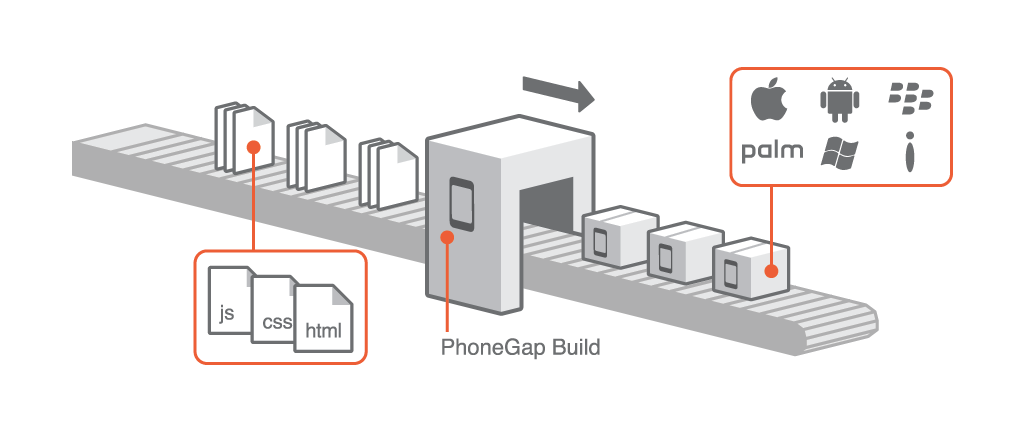
\includegraphics[scale=0.4]{imagens/PHONEGAP}
	\subcaption{\textbf{Fonte:} \citeauthorandyear{IONIC2017_ADRIAN_GOIS}}
	\label{fig:figura3}
\end{figure*}
\FloatBarrier

A programação com base em \textit{PhoneGap/Cordova} por meio de tecnologias de \textit{front-end}, torna possível a concepção (\textbf{\textit{build}}) de aplicações móveis nativas para as plataformas \textbf{alvo}, esses aplicativos desempenham características semelhantes aos programas nativos, pois o \textit{software} está sendo compilado incorporado em uma  espécie de navegador de internet, denominado de \textit{webview}, porém, essa abstração com o navegador \textit{webview} é invisível e imperceptível para os seus utilizadores. Esse navegador adaptado beneficia-se primordialmente da linguagem de marcação \textit{HTML}, de uma folha de formatação de estilo \textit{CSS} e do \textit{JavaScript} para sua exibição e funcionamento \cite{IonicCordovaMedium2017}. Para criar-se uma aplicação compatível com mais de um sistema operacional com o \textit{IONIC Framework}, faz-se necessária a instalação do \textit{IONIC Framework CLI}, \textit{JDK} versão 7, \textit{SDK do Android}, \textit{NodeJS} e um editor de texto ou \textit{IDE} compatível \cite{IONIC2017_ADRIAN_GOIS}.

\subsection{Linguagem \textit{Kotlin}}
%pagi dona 38
Em 2017, foi divulgado que seria possível desenvolver aplicações móveis nativas voltadas para o sistema operacional \textit{Android} utilizando não somente a linguagem \textit{Java}, mas também desenvolver com \textit{Kotlin}, todo o público presente no evento \textit{Google I/O} apoiou e aprovou o pronunciamento. Com tal possibilidade de se escolher entre as duas linguagens e até mesmo mesclá-las nos mesmos projetos, classes e afins, o desenvolvimento \textit{Android} tornou-se muito mais proveitoso \cite{Lecheta2018}.

A motivação para criação do Kotlin foi basicamente suprir as necessidades encontradas pela equipe da JetBrains durante os anos de desenvolvimento de ambientes integrados como \textit{IntelliJ}, \textit{PyCharm}, \textit{RubyMine} e \textit{WebStorm} usando \textit{Java} como linguagem principal e também \textit{Scala}. A linguagem foi batizada com o nome da ilha Russa de \textit{Kotlin} localizada próxima a São Petersburgo \cite{Lecheta2018}.

%pagina 38
Tanto \textit{Kotlin} como o  \textit{Android Studio} que é a  \textit{IDE} oficial de desenvolvimento  \textit{Android}, foram criados pela empresa russa  \textit{JetBrains}. Sua sintaxe de fácil compreensão proporciona uma programação mais prazerosa. Possui total compatibilidade com a linguagem \textit{Java} pois ambas utilizam a \textit{JVM} \cite{Lecheta2018}.

% cap 1.1
A linguagem começou a ser desenvolvida em 2011, com base no vasto conhecimento da empresa \textit{JetBrains} no desenvolvimento e suporte de \textit{IDE's} tanto para \textit{Java} como para vários outros tipos de tecnologias, com a intenção de chegar-se a uma linguagem que poderia ser executada e/ou usada nos mesmos projetos onde \textit{Java} era utilizado e não somente para o ecossistema \textit{Android}\footnote[4]{O ecossistema Android é composto pelas linguagens suportadas pela \textit{JVM} referente a programação Android nativa, ambiente (\textit{IDE}) e kit de desenvolvimento e a loja oficial na qual os aplicativos são disponibilizados \cite{EcossitemaAndroid}}. Em meados de 2006, já havia a possibilidade de se realizar o \textit{download} do complemento e instalar na \textit{IDE Android Studio} para programar em \textit{Kotlin} para \textit{Android} \cite{Resende2018}. 

A seguir os pontos que tornam a linguagem tão relevante no mercado de desenvolvimento \cite{Resende2018}:

\begin{itemize}
% cap 1.4
\item \textbf{Sucinta:} A característica de ser uma linguagem com sintaxe bem sucinta em relação ao \textit{Java}, significa que ao converter um arquivo/classe \textit{Java} para \textit{Kotlin} o resultado final será o mesmo, porém em uma abordagem com \textit{Kotlin} teria-se menos códigos desnecessários, como uma classe sem métodos acessores e modificadores explícitos por exemplo, o que facilita em muito a leitura e manutenção de código, essa conversão pode ser realizada tanto de forma manual ou com recursos da própria \textit{IDE Android Studio}. %\cite{Resende2018}.

% cap 1.5 ??
\item \textbf{Protegida contra exceções:} Uma das exceções mais encontradas na programação \textit{Java}, com certeza é \textit{NullPointerException} que se trata de uma menção a algo que ainda não está disponível a nível  de programa. Em \textit{Kotlin} \textbf{não} é possível atribuir o valor nulo a uma variável, para forçar uma variável a receber um valor nulo é necessário adicionar um \textbf{ponto de interrogação} na declaração do tipo. %\cite{Resende2018}. 

\item \textbf{Desejada:} 2º linguagem de desenvolvimento mais querida, a 4º mais pesquisada e a 22º mais admirada do ano de 2018, segundo pesquisa realizada com mais de 100 mil usuários de todas as partes do mundo. %\cite{StackOverFlow2018}.

\item \textbf{Integrada:} Desde a versão 3.0 da \textit{IDE Android Studio}, fez-se desnecessária a instalação de \textit{plugins Kotlin}, pois o complemento passou a ser disponibilizado totalmente integrado com o ambiente de desenvolvimento.% \cite{Teodosio}.

% cap 1.3
\item \textbf{Compatível\footnote{ \textit{\textbf{ART} Android Runtime}: Ambiente de tempo de execução a partir do \textit{Android} 5 e superior.
\textit{\textbf{DALVIK} Android Runtime}: Ambiente de tempo de execução em versões inferiores ao \textit{Android} 5. \cite{ArtDalvik}}:} A total compatibilidade entre a linguagem da empresa \textit{JetBrains} e \textit{Java}, permite a troca de dados entre arquivos tanto na extensão .kt como .java. %\cite{Resende2018}. 
\end{itemize}

Os arquivos que possuem extensão .kt foram desenhados e idealizados desde sua concepção para possibilitarem sem maiores dilemas e complicações inúteis as chamadas aos arquivos de extensão .java de forma totalmente nativa e eficaz, conforme apresentado na Figura 6. %\cite{JetbrainsDocs}

\FloatBarrier
\begin{figure*}[!htbp]
	\centering
		\caption{Fluxo de conversão de códigos Kotlin e Java para \textit{bytecode}} 
	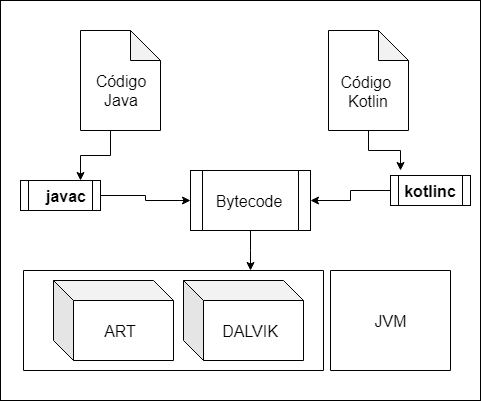
\includegraphics[scale=0.5]{imagens/androidKotlinJVM}
\subcaption{\textbf{Fonte:} Adaptado pelo autor} - \cite{SlideShare}
	\label{fig:figura4}
\end{figure*}
\FloatBarrier


\section{Qualidade de Código}
Qualquer profissional da área de tecnologia e programação tem plena de consciência da qualidade dos seus códigos, porém, em projetos consideravelmente maiores, e com muitos responsáveis, pode ocorrer a perda da qualidade no projeto. Para sanar essas adversidades, existem diversos programas, que realizam de forma automática ou não, o controle e a análise de qualidade, produzindo relatórios técnicos, entretanto, nem sempre se chega ao resultado esperado \cite{qualidadedesoftware}. 

\subsection{Refatoração de Código}
A técnica de refatoração propõe examinar os códigos já existentes, com o objetivo de se reduzir repetições (desnecessárias) e incoerências presentes no sistema \cite{lindstrom2017refatoracao}. Com a falta da prática de se refatorar, os projetos acabam tornando-se muito complexos, inviabilizando futuras alterações e correções, chegando ao ponto de se cogitar a total reescrita de um sistema, independente do seu tamanho e importância. Em seu livro Código Limpo, o renomado autor Robert C. Martin definiu alguns parâmetros para uma refatoração eficiente \cite{ZanetteBeCodeCleanCode2017}: 

\begin{itemize}
\item{\textbf{Nomenclaturas}}:
Deve-se declarar operações, propriedades, parâmetros e classes de forma condizente com sua função, para que  ao realizar a leitura, seja fácil identificar o seu verdadeiro propósito. As nomenclaturas devem ser as mais fiéis possíveis, mesmo que para se alcançar o objetivo, seja necessária uma nomenclatura relativamente grande. Operações necessitam obrigatoriamente serem declaradas com nomenclatura de verbos, e classes e suas instâncias necessitam estar declaradas como substantivos \cite{ZanetteBeCodeCleanCode2017}.

\item{\textbf{Operações}}:
Robert C. Martin, diz que as operações devem ser curtas e descomplicadas, o quanto menor for uma operação, melhor. Uma operação só pode executar exclusivamente uma atividade, isso vai oportunizar o reaproveitamento da operação, dessa forma será mais fácil a revisão e conservação do código \cite{ZanetteBeCodeCleanCode2017}.

\item{\textbf{Comentários/Anotações}}:
Deve-se comentar o mínimo possível, pois apesar dos sistemas estarem sempre em modificações, os comentários acabam sendo esquecidos e pode vir a prejudicar futuramente. Portanto ao utilizá-lo, deve ser sempre revisado \cite{ZanetteBeCodeCleanCode2017}.

\item{\textbf{Duplicidades}}:
Cada parte de compreensão do código, necessita ser exclusiva, pois é prejudicial trechos semelhantes de código que executam a mesma operação em lugares diferentes, pois torna-se muito mais difícil e passível de esquecimento realizar uma mesma modificação em múltiplos locais dentro de um programa. Mesmo que nem toda duplicidade afete razoavelmente, aconselha-se livrar-se delas \cite{ZanetteBeCodeCleanCode2017}.

\item{\textbf{Prevenção}}:
Deve-se aproveitar ao máximo os recursos de tratamentos e exceções e erros, oferecidos pela maioria das linguagens de programação disponíveis, tomando \textit{Java} como exemplo, temos disponíveis \textit{Exceptions} e blocos \textit{try-catch}. Um sistema necessita estar pronto para as situações adversas das idealizadas por seu criador. Orienta-se também, evitar os valores nulos em qualquer parte, sempre que possível \cite{ZanetteBeCodeCleanCode2017}.

\item{\textbf{Reescrita}}:
Deve-se criar a rotina de reescrita de código, com isso o sistema estará sempre atual, o ideal é reescrever enquanto a raciocínio utilizado ainda está recente na mente do desenvolvedor, mas deve-se tentar evitar sempre a criação de possíveis novos \textit{bugs} \cite{ZanetteBeCodeCleanCode2017}. 

\item{\textbf{Verificação}}:
Os testes de \textit{software} necessitam ser eficazes, ágeis, individuais, sem duplicidades e efetuar sempre a operação que para a qual foi-se desenhado e programado para realizar. Orienta-se a aplicação do \textit{TDD}, ou seja, primeiro criando a operação de testes, em seguida o trecho de código a ser verificado e após a conclusão, deve-se refatorar \cite{ZanetteBeCodeCleanCode2017}.

\end{itemize}

\subsection{Ferramentas para Análise de Qualidade de Código}

Entende-se por Analisadores Estáticos de Códigos (AEC), os programas capazes de identificar, enumerar e até mesmo solucionar imperfeições e falhas existentes em um \textit{software}, o que possibilita que desenvolvedores e gerentes de projeto preocupem-se com outros fatores de um sistema, uma vez que se tem uma ferramenta específica para realização de uma análise mais detalhada \cite{AECMedium2018}. 

Com a utilização de um AEC, as falhas e possíveis ameaças são prontamente detectadas, e isso é realizado dentre outras funcionalidades pela análise de:

\begin{itemize}
    \item \textbf{Quantidade de linhas de código} (\textit{Lines of code} - \textit{LOC}) utilizadas, o que pode variar de acordo com as linguagens de programação (mais ou menos verbosas) empregadas no projeto \cite{DevQA}.
    
    \item {\textbf{Quantidade de instruções condicionais e de repetição} (\textit{Cyclomatic Complexity} - \textit{CC}) aconselha-se que esse número seja sempre o mais baixo possível segundo Robert C. Martin, autor do livro \textit{Clean Code}. \cite{DevQA}.}
    
    \item{\textbf{Coerência das operações} (\textit{Lack of Cohesion of Methods} - \textit{LCOM}) no qual são quantificadas as responsabilidades exercidas pelo conteúdo de uma classe. \cite{DevQA}.}
\end{itemize}

\subsubsection{\textit{SonarQube}}
Anteriormente chamado apenas de \textit{Sonar}, o \textit{SonarQube} desenvolvido pela \textit{SonarSource SA}, é um sistema \textit{web} de código fonte aberto que realiza a verificação das características de um programa e exibe os resultados obtidos por meio de um painel \cite{AECMedium2018}, conforme Figura 7. Dentre suas muitas possibilidades de análise, destacam-se as verificações de padrões de projeto, duplicidade de código e prevenção contra as possíveis inconsistências \cite{DevQA}.

Além de ser personalizável ao gosto do usuário, o programa oferece ainda a possibilidade de ser utilizado juntamente com diversos ambientes de desenvolvimento integrado disponíveis no mercado e também com sistemas de versionamento de projeto como o \textit{GitHub} da \textit{Microsoft}, possibilitando uma oportunidade para efetuar-se correções e ajustes de problemas antecedendo futuras alterações e problemas relacionados ao versionamento \cite{DevQA}. 

\FloatBarrier
\begin{figure*}[!htbp]
	\centering
		\caption{Parte do Painel do \textit{SonarQube}} 
	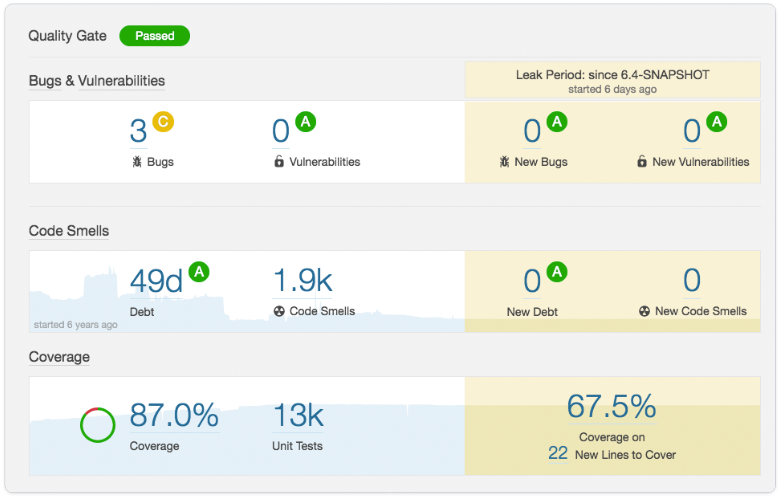
\includegraphics[scale=0.6]{imagens/SONAR2}
  \subcaption{\textbf{Fonte:} \cite{SonarSite}}
	\label{fig:figura7}
\end{figure*}
\FloatBarrier

\subsubsection{\textit{Ebert}}

 O \textit{Ebert} é um sistema pago e desenvolvido pela \textit{Caliper Metrics} parte da empresa brasileira Plataformatec que provê uma análise tanto estática como contínua dos códigos desempenhados, por meio de uma total integração com o sistema versionamento de projetos \textit{GitHub}, com a sua utilização a equipe torna-se muito mais apta para visualizar os erros, recebendo sugestões para solução e também dicas para desviar-se deles pelo decorrer de todo o projeto. O sistema abstrai dos envolvidos a necessidade de uma verificação de alterações de códigos submetidos para entrar em produção, notificando instantaneamente sobre brechas de segurança, duplicidades, incoerências desnecessárias, incompatibilidades e também permite vários ajustes e modificações referentes às verificações de código apresentadas, conforme apresentado na Figura 8 \cite{Ebert}.
 
 \FloatBarrier
\begin{figure*}[!htbp]
	\centering
		\caption{Interface do \textit{Ebert}} 
	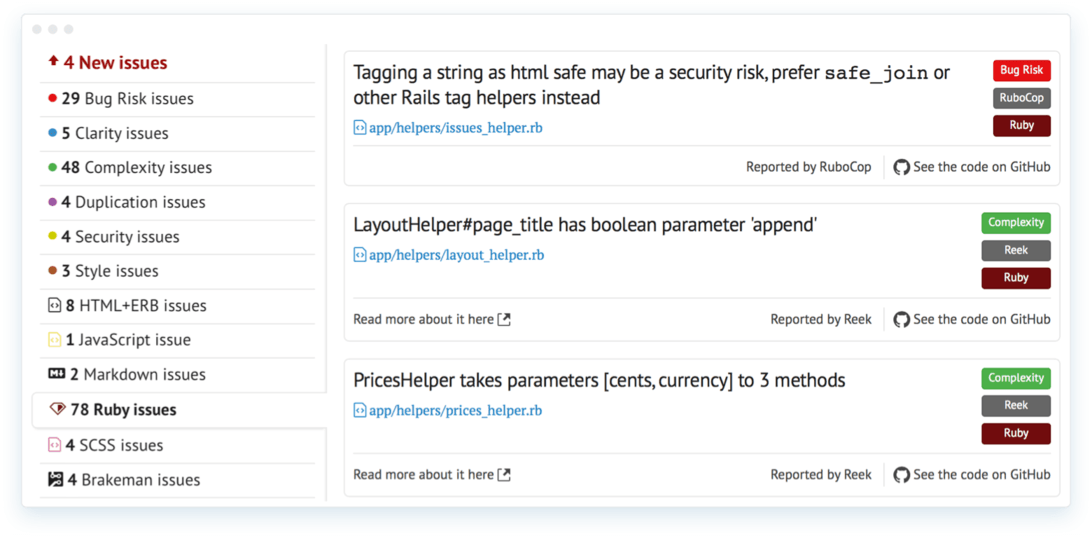
\includegraphics[scale=0.4]{imagens/Ebert}
  \subcaption{\textbf{Fonte:} \cite{Ebert}}
	\label{fig:figura7}
\end{figure*}
\FloatBarrier

\section{Trabalhos Relacionados a esta Pesquisa}

Nesta subsecção, serão apresentados alguns trabalhos relacionados ao tema principal da pesquisa: a linguagem de programação \textit{Kotlin} e a qualidade de \textit{software} por meio de técnicas e tecnologias.

\subsection{Desenvolvimento de Aplicativo para Adoção de Animais Abandonados Utilizando a Linguagem de Programação \textit{Kotlin} e Programação Reativa \cite{TccKotlin}}

O intuito do trabalho realizado na Universidade Tecnológica Federal do Paraná nos Departamentos de Acadêmicos de Eletrônica e Informática no curso Engenharia da Computação é de se minimizar o número de animais desabrigados nas grandes cidades como Curitiba, com a criação de uma aplicação móvel nativa, destinada para usuários do sistema operacional \textit{Android}, utilizando os recursos oferecidos pela linguagem de programação \textit{Kotlin} para obter-se mais uma opção para auxiliar as ferramentas já existentes destinadas a facilitar o encontro e a adoção dos animais de rua \cite{TccKotlin}.

Apesar das dificuldades em utilizar algumas tecnologias de armazenamento de dados mais atuais como o \textit{Firebase}, as metas desejadas foram alcançadas com a criação de uma aplicação móvel em uma linguagem de desenvolvimento ainda pouco conhecido para os meios acadêmicos mas que ofereceu inúmeros aspectos que facilitaram em muito a programação, o projeto encabeçou aumentar a integração das \textit{ONG's} com os interessados em adoção. Como ideia para próximos passos ficaram a criação de um sistema destinado para usuários do sistema operacional \textit{iOS} e a resolução de alguns \textit{bugs} simples, mas que facilitaram a usabilidade do sistema. No decorrer do desenvolvimento da pesquisa, \textit{Kotlin} passou a ser a nova linguagem de desenvolvimento oficial para \textit{Android} \cite{TccKotlin}. 

\subsection{\textit{Framework} para Avaliação da Qualidade de Código: Uma
Abordagem Baseada em Valor \cite{Framework}}
A meta da pesquisa realizada na Universidade de Brasília, era a análise e o acompanhamento de algumas metodologias denominadas ágeis, juntamente com técnicas de testes de unidade de \textit{software} para obtenção de sistemas menos propensos a futuro/possíveis erros provenientes da falta de averiguação por parte dos envolvidos \cite{Framework}. 

Com o cumprimento da meta geral e das específicas como primeira etapa do trabalho, nessa fase inicial da pesquisa, foram planejados todos os possíveis passos para aplicação e utilização do \textit{framework ágil} \textit{Scrum} e/ou \textit{XP} e dos testes de unidade, com intuito de resultar em melhores acabativas nos projetos desempenhados pela  Controladoria Geral do Distrito Federal e do Laboratório Fábrica de \textit{Software} - Campus UnB Gama, ambos localizados em Brasília. Nas etapas futuras, planeja-se colocar em prática os conceitos idealizados \cite{Framework}.

\subsection{Proposta de Plano de Garantia da Qualidade de \textit{Software} para o Laboratório de
Criação e Aplicação de \textit{Software} \cite{PropostaDePlano}}

Neste artigo desenvolvido na Universidade de Caxias do Sul - Centro de Computação e Tecnologia da Informação, tinha-se como objetivo para a pesquisa, analisar as atuais técnicas de programação empregadas no Laboratório de Criação e Aplicação de \textit{Software} da instituição, para que através dessa futura análise torna-se possível implementar pelo menos parte das ferramentas e técnicas corretas com o propósito de garantir que todos os programas desenvolvidos obtivessem maior qualidade em suas entregas, tanto para os programadores, quanto para os responsáveis técnicos pelos projetos e principalmente para os utilizadores finais. \cite{PropostaDePlano}.

Os propósitos da pesquisa foram cumpridos, mediante acompanhamento e implantação de ferramentas abertas para gerir o processo de desenvolvimento por parte dos programadores, evidenciou-se que é praticamente impossível realizar um desenvolvimento sem imperfeições e defeitos. Para trabalhos futuros, indicou-se a elaboração de uma inspeção para maiores reconhecimentos dos ganhos obtidos \cite{PropostaDePlano}.

\subsection{Estimando Atributos de Qualidade de \textit{Software}
Utilizados e Desejados pelas Empresas
Certificadas no \textit{MPS-SW} no Brasil \cite{EstimandoAtributos}}

Nesta pesquisa desenvolvida na Universidade Federal de Ouro Preto, Departamento de Computação e Sistemas, Colegiado de Engenharia de Computação, o intuito era de se elaborar uma equiparação entre a característica dos programas e sistemas entregues e características almejadas pelas empresas participantes do estudo \cite{EstimandoAtributos}.

Alcançou-se o objetivo do trabalho, mesmo com da falta de comprometimento das empresas solicitadas em se envolverem e responderem algumas perguntas e questionários simples. Constatou-se que as empresas na sua maioria, contam com metodologias ágeis no seu dia-a-dia de programação e mais instrumentos automáticos que por sua vez, executam a geração e o acompanhamento de métricas referentes às tarefas desempenhadas, principalmente os códigos desenvolvidos. \cite{EstimandoAtributos}.

\chapter{Metodologia}
\label{cap:03}

Para que seja possível cumprir os objetivos desse trabalho de conclusão de curso, no presente capítulo serão apresentados todos os passos a serem desenvolvidos. Todos os trechos de código utilizados nesta seção para comparação entre as linguagens \textit{Kotlin} e \textit{Java} apresentam-se disponíveis para visualização e consulta no sistema de gerenciamento e versionamento de projetos \textit{GitHub} no endereço \url{https://github.com/wendreof/tcc}.

Para a organização dos códigos utiliza-se as formatações, endentações e otimização de importações oferecidas pela própria \textit{IDE Android Studio} e para a estruturação dos projetos utiliza-se o padrão de desenvolvimento com nomenclatura de classes, variáveis, operações e relacionados somente na língua inglesa. Em cada um dos experimentos, explica-se de forma resumida o conteúdo de cada trecho de código, e as particularidades referentes, principalmente ao \textit{Kotlin}, pois o presente trabalho não tem por objetivo, se aprofundar em todos os conceitos relacionados às tecnologias aplicadas.

Todos os comentários utilizados nos trechos de códigos no decorrer do capítulo, apresentam-se sem seus devidos acentos e pontuações, devido a falta de compatibilidade com o Formato de Transformação Unicode 8-bit (\textit{Unicode Transformation Format – 8-bit - UTF-8}).

\section{Panorama Geral da Pesquisa}

O panorama geral desta pesquisa, conforme representado a seguir na Figura 9, propõe-se a esclarecer o motivo da escolha da apresentação de uma nova tecnologia para o desenvolvimento de \textit{software} voltado para os dispositivos móveis por meio de métricas para comparação entre duas linguagens de programação, sendo elas \textit{Java} e \textit{Kotlin}, que por sua vez fazem parte do ecossistema da plataforma móvel \textit{Android} e o desenvolvimento e análise de experimentos baseados em trechos de códigos que desempenham as mesmas funcionalidades.

\FloatBarrier
\begin{figure*}[!htbp]
	\centering
		\caption{Panorama Geral da Pesquisa}
	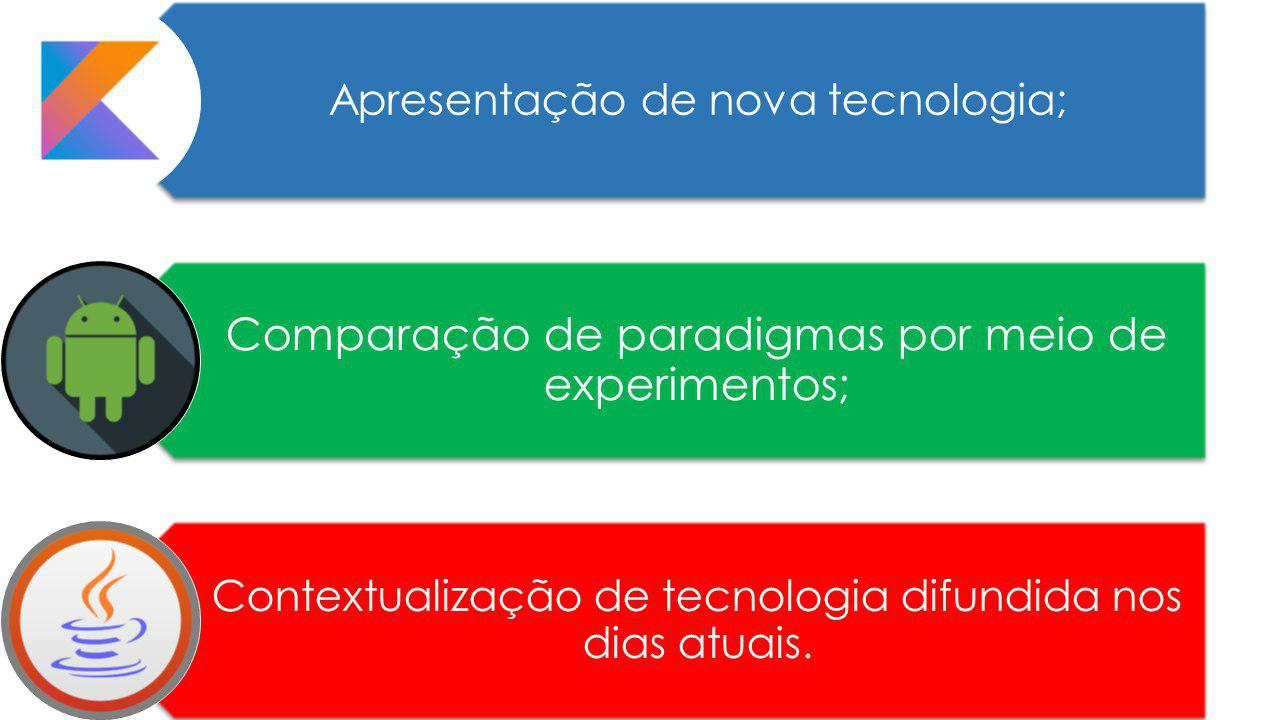
\includegraphics[scale=0.5]{imagens/metodologia1}
	\subcaption{\textbf{Fonte:} Elaborado pelo autor}
	\label{fig:figura3}
\end{figure*}
\FloatBarrier

De acordo com o panorama geral da pesquisa, apresentado na Figura 9 acima, a seguir listam-se todas as etapas a serem operacionalizadas, para cumprir-se os objetivos gerais e específicos deste trabalho de conclusão de curso.

\begin{itemize}
    \item \textbf{Etapa 01}: Justificativa para Adoção do \textit{Kotlin} com Destaque nos Aspectos de Usabilidade;
    
    \item \textbf{Etapa 02}: Métricas de Usabilidade para Comparação;
    
   \item \textbf{Etapa 03}: Definição de Experimentos para Comparação entre \textit{Kotlin} e \textit{Java};

   \item \textbf{Etapa 04}: Comparação entre as Linguagens Kotlin e Java para os Experimentos Definidos.
\end{itemize}

\section{Etapas para o Desenvolvimento da Pesquisa}

\subsection{Etapa 01: Justificativa para Adoção do \textit{Kotlin} com Destaque nos Aspectos de Usabilidade}

Como reforçado nos capítulos anteriores dessa pesquisa, mais especificamente no segundo capítulo, a linguagem de programação Java ainda é o principal e mais utilizada para desenvolvimento de aplicações móveis destinadas para os usuários do sistema operacional \textit{Android}. Desde seu anúncio oficial, o \textit{Kotlin} chegou para oferecer aos desenvolvedores mais uma opção no momento de escolha de tecnologias para elaboração de novos aplicativos assim como a manutenção de sistemas legados, ou seja, \textit{Kotlin} não vai e nem pretende substituir o \textit{Java}, mas sim \textbf{coexistir} de forma homogênea no ecossistema \textit{Android}. Munido de recursos mais modernos, inspirados em tecnologias reconhecidas no mercado de desenvolvimento de software, com \textit{Kotlin} torna-se possível escrever algoritmos compreendidos pela \textit{JVM}, de modo mais simples, facilitando todas as etapas que envolvem a programação e possibilitando o aproveitamento de tudo que já foi escrito em \textit{Java} como classes, projetos e bibliotecas.

Ao término da pesquisa, pretende-se evidenciar as vantagens da programação com foco em dispositivos móveis, utilizando como principal tecnologia, a linguagem de programação \textit{Kotlin}, apoiando-se em seus aspectos modernos e enxutos, resultando em uma menor quantidade de código clichê e desnecessário que em nada auxiliam a aplicação e acabam dificultando a manutenção.

\subsection{Etapa 02 - Métricas de Usabilidade para Comparação} 
Baseando-se em um dos conceitos descritos pelo escritor e engenheiro de \textit{software} americano Robert C. Martin, autor do renomado livro \textit{Clean Code: A Handbook of Agile Software Craftsmanship}, no qual se é descrito que na programação lê-se muito mais vezes do que se escreve um código propriamente dito, as etapas estabelecidas para equiparar \textit{Kotlin} e \textit{Java} são apresentadas na Tabela 2:

\FloatBarrier
\begin{table}[!htbp]
\centering
\caption{Métricas de comparação}
	\begin{tabular}{ c | c }
		\hline
		\textbf{Métrica} & \textbf{Definição}                  \\ \hline
		
		             1 	 & Quantidade de caracteres utilizados	\\ \hline
		             
		             2   & Quantidade de linhas de código        \\ \hline
		             
		         	 3   & Tamanho do arquivo em quilobytes (Kb) \\ \hline
	\end{tabular}
	\\ \vspace{0.2cm}
	\textbf{Fonte:} Elaborada pelo autor
	\label{tab:exemplo}
\end{table}
\FloatBarrier

%\begin{itemize}
%\    \item \textbf{Quantidade de caracteres}: Em uma linguagem de programação mais verbosa utiliza-se uma quantidade relativamente maior de caracteres e símbolos
    
%\     \item \textbf{Quantidade de linhas de código}: Em um código considerado verboso, encontra-se uma quantidade maior de palavras e/ou palavras mais longas para se expressar a intenção do algoritmo (consequentemente mais linhas)

%\     \item \textbf{Tamanho do arquivo em Quilobytes (Kb)}: Quanto maior o tamanho do arquivo (.java/.kt), maior será o tempo utilizado para ser efetuada a compilação pela \textit{JVM} %\\end{itemize}  

Em linguagens de programação mais verbosas, faz-se necessária a utilização de uma maior quantidade de caracteres e símbolos, da mesma forma podem-se aumentar a quantidade de palavras chaves e palavras mais longas que o normal para que se torne possível se expressar a real intenção de um algoritmo, o que gera a inclusão de mais linhas no projeto, e consequentemente aumenta o tamanho final do arquivo utilizado em caso de linguagens compiladas como o \textit{Java} e sua \textit{JVM}. Entende-se que uma determinada linguagem que necessita de menos de caracteres, expressões e linhas de código é menos verbosa, mais expressiva e de maior facilidade referente a sua manutenção.

Assim, para os experimentos desta pesquisa, ao comparar as linguagens \textit{Kotlin} e \textit{Java}, serão analisadas as métricas apresentadas na Tabela 2.

\subsection{Etapa 03 - Definição de Experimentos para Comparação entre \textit{Java} e \textit{Kotlin}}

Abaixo os experimentos a serem desenvolvidos no decorrer do capítulo para que seja possível atingir o objetivo de comparação:

\textbf{Experimento I} - \textit{Hello World}!: Apresentação de um pequeno trecho de código que ao ser executado, apresenta uma saída para o usuário;

\textbf{Experimento II} - Operação Aritmética Básica: Elaboração de uma função que tem por intuito realizar a somar de dois números inteiros e interpolar o resultado com um texto;

\textbf{Experimento III} - Classe \textit{Student}: Implementação de uma classe modelo que abstrai algumas das características presentes em um estudante;

\textbf{Experimento IV} - Classe \textit{ThermometricScale}: Apresentação da classe base para o desenvolvimento da aplicação de medidas termométricas e declaração de suas três funções;

\textbf{Experimento V} - Interface \textit{Temperature}: Implementação de uma interface e um método que recebe dois valores por parâmetros e retorna um único valor;

\textbf{Experimento VI} - Classe \textit{Adapter}:
Utilização das técnicas de se extender e implementar uma classe e uma interface;

\textbf{Experimento VII} - \textit{Activity Main}: Criação da principal classe da aplicação de conversão e implementação de todos os eventos de clique e substituição dos textos apresentados na interface.

Nos experimentos I, II, II trabalham-se trechos desconexos de códigos de caráter mais introdutórios das duas linguagens, entretanto, nos experimentos IV, V, VI e VII com o intuito de aprofundar-se mais especificamente na plataforma \textit{Android} e no seu ecossistema, apresentam-se duas classes, uma interface e uma terceira classe do tipo \textit{activity}, ambas referentes a uma aplicação que realiza a conversão de valores termométricos de acordo com o diagrama em Linguagem de Modelagem Unificada (\textit{Unified Modeling Language} - \textit{UML}) apresentado na Figura 10:

\FloatBarrier
\begin{figure*}[!htbp]
	\centering
		\caption{Diagrama \textit{UML} de Aplicação de Conversão de Medidas Termométricas}
	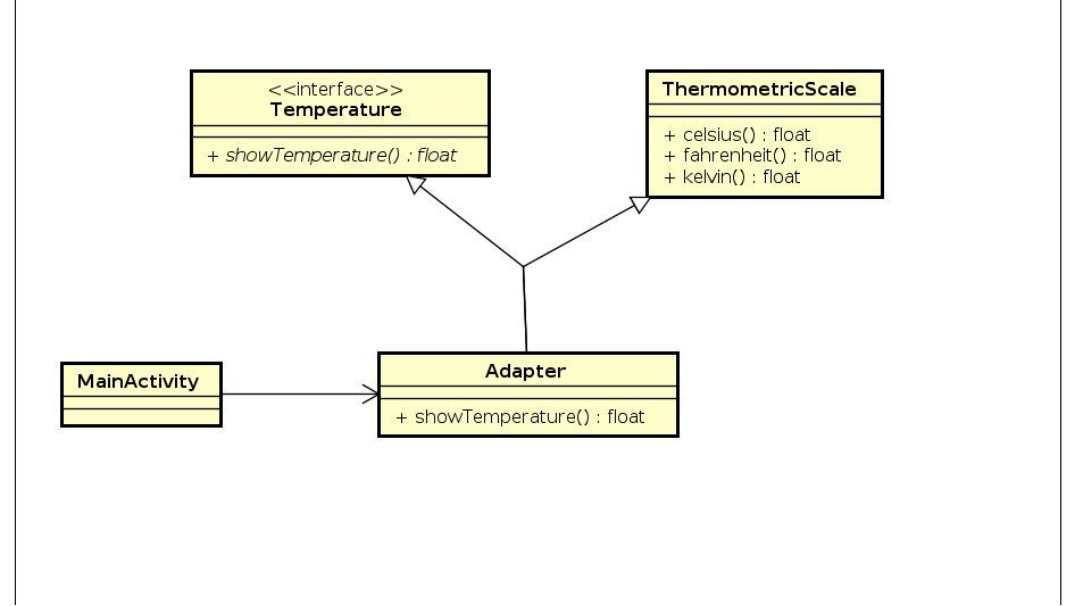
\includegraphics[scale=1]{imagens/umlTCC}
	\subcaption{\textbf{Fonte:} Elaborado pelo autor}
	\label{fig:figura3}
\end{figure*}
\FloatBarrier

No diagrama \textit{UML} disponibilizado na Figura 10 acima, apresenta-se um exemplo de implementação do padrão de projeto \textit{Adapter} em uma aplicação móvel, na Tabela 3 detalha-se cada uma das classes e suas respectivas funções:

\FloatBarrier
\begin{table}[!htbp]
\centering
\caption{Classes e Definições do diagrama UML - Figura 10}
	\begin{tabular}{ c | c }
		\hline
		\textbf{Classe} & \textbf{Definição}\\ \hline
		
         \textit{Adapter} & Adaptar a interface \textit{Temperature} e a classe \textit{ThermometricScale}
         \\ \hline
         
          \textit{Temperature}   & Definir a interface de domínio específica a ser adaptada
          \\ \hline
         
     	 \textit{MainActivity}  & Colaborar com objetos da a interface \textit{Temperature}
     	 \\ \hline
     	 
     	   \textit{ThermometricScale}  & Definir uma interface existente que necessita ser adaptada
     	   \\ \hline
	\end{tabular}
	\\ \vspace{0.2cm}
	\textbf{Fonte:} Elaborada pelo autor
	\label{tab:exemplo}
\end{table}
\FloatBarrier

\subsection{Etapa 04 - Comparação entre as Linguagens \textit{Kotlin} e \textit{Java} para os Experimentos Definidos}

\subsubsection{Experimento I - \textit{Hello World!}}

Como início da comparação, apresenta-se nessa subseção, duas versões de um \textit{Hello World}, que nada mais é, do que um trecho de código básico que normalmente é empregado de forma educacional para iniciantes para se exemplificar os princípios de uma determinada linguagem. A função de um \textit{Hello World} é exibir o texto \textit{Hello World!} (Olá Mundo!) de forma visual por meio de uma saída, seja ela \textit{IDE}, terminal ou tela.

Em versões anteriores do \textit{Kotlin}, fazia-se necessária a implementação de um parâmetro do tipo \textit{Array} de \textit{Strings} na função \textit{main} assim como faz-se necessário em \textit{Java}.


Exemplo de implementação de \textit{Hello World} em \textit{Kotlin}
\caption{Hello World em Kotlin}
\lstinputlisting[language=kotlin]{fontes/Main.kt} 

Exemplo de implementação de \textit{Hello World} em \textit{Java}
\caption{Hello World em Java}
\lstinputlisting[language=java]{fontes/Main.java} 


\subsubsection{Experimento II - Operação Aritmética Básica}

Nessa subseção, apresentam-se duas formas de se implementar a função aritmética de soma, declarando-se uma variável inteira que recebe a soma de dois valores inteiros, sendo eles os números 99 e 1 respectivamente, obtendo-se um total de 100. Os trechos de código após execução exibem um texto concatenando com a variável que recebeu o valor da soma.

Em Kotlin disponibilizam-se para utilização dois tipos de variáveis, sendo eles as variáveis mutáveis do tipo \textbf{\textit{var}} que podem ter seus valores alterados ao decorrer da execução do programa e as variáveis imutáveis do tipo \textbf{\textit{val}} que podem receber apenas uma atribuição de valor, sendo assim variáveis finais.

Exemplo de implementação de função aritmética de soma em \textit{Kotlin}
\caption{\textit{Hello World} em \textit{Kotlin}}
\lstinputlisting[language=Kotlin]{fontes/Operations.kt} 

Exemplo de implementação de função aritmética de soma em \textit{Java}
\caption{Hello World em Java}
\lstinputlisting[language=java]{fontes/Operations.java} 


\subsubsection{Experimento III - Classe \textit{Student}}

Nessa subseção foram implementam-se de formas diferentes uma mesma versão de uma classe \textit{Student} na qual implementam-se quatro atributos, sendo eles um atributo name do tipo \textit{string}, outro atributo denominado \textit{tccTitle} também do tipo \textit{string}, \textit{approved} do tipo \textit{boolean} e \textit{yearsOld} do tipo \textit{integer}, e as operações disponíveis são métodos acessores e de configuração \textit{getters} e \textit{setters}, \textit{toString}, \textit{equals} e \textit{hashCode}, todos eles comumente usados em classes do tipo \textit{Model} e na programação \textit{Java}.

Classes do tipo \textit{data class}  já possuem por padrão os métodos \textit{getter}, \textit{setter}, \textit{toString}, \textit{equals}, \textit{hashCode} e \textit{copy} implícitos, tornado desnecessária em \textit{Kotlin} a re-implementação das funções. Para obter-se um resultado parecido em \textit{Java} seria necessário configurar o \textit{Project Lombok} e utilizar as anotações \textit{@Getter}, \textit{@Setter}, \textit{@ToString} e \textit{@EqualsAndHashCode} ou a anotação \textit{@Data} no início da implementação da classe ou alguma outra ferramenta com o mesmo propósito.

Exemplo de implementação de uma classe \textit{Student} em \textit{Kotlin}
\caption{Exemplo de implementação de uma classe \textit{Student} em \textit{Kotlin}}
\lstinputlisting[language=kotlin]{fontes/Student.kt} 

Exemplo de implementação de uma classe \textit{Student} em \textit{Java}
\caption{Exemplo de implementação de uma classe \textit{Student} em \textit{Java}}
\lstinputlisting[language=java]{fontes/Student.java} 

\subsubsection{Experimento IV - Classe \textit{ThermometricScale}}

A classe \textit{ThermometricScale} não possui atributos, apenas três funções, sendo elas \textit{celsius}, \textit{fahrenheit} e \textit{kelvin}, cada uma das operações recebe e retorna um único valor do tipo \textit{float} que é utilizado na fórmula específica de cada uma das escalas termométricas implementadas.

Em \textit{Kotlin} é possível declarar uma função, seu tipo e respectivo retorno na mesma linha de forma mais simplificada e enxuta.

Classe \textit{ThermometricScale} em \textit{Kotlin}
\caption{\textit{ThermometricScale} em \textit{Kotlin}}
\lstinputlisting[language=kotlin]{fontes/ThermometricScaleKotlin.kt} 

Classe \textit{ThermometricScale} em \textit{Java}
\caption{\textit{ThermometricScale} em Java}
\lstinputlisting[language=java]{fontes/ThermometricScaleJava.java}

\subsubsection{Experimento V - Interface \textit{Temperature}}

A interface \textit{Temperature} possui apenas um único método denominado de \textit{viewTemperature}, que recebe por parâmetro um valor também do tipo \textit{float} e um único caractere.

Interface \textit{Temperature} em \textit{Kotlin}
\caption{Interface \textit{Temperature} em Kotlin}
\lstinputlisting[language=kotlin]{fontes/TemperatureKotlin.kt} 

Interface \textit{Temperature} em \textbf{\textit{Java}}
\caption{Interface \textit{Temperature} em \textit{Java}}
\lstinputlisting[language=java]{fontes/TemperatureJava.java} 


\subsubsection{Experimento VI - Classe \textit{Adapter}}

Na classe \textit{Adapter} implementada em \textit{Java}, torna-se necessária a criação da variável auxiliar r do tipo \textit{Float}, para que seja possível atribuir e retornar ao final da estrutura de decisão condicional \textit{Switch} o valor de forma correta. No entanto, na implementação em \textit{Kotlin}, a própria estrutura \textit{When} responsabiliza-se em retornar por padrão um valor, dispensando a criação de uma variável auxiliar.

A expressão \textit{when} está para a linguagem \textit{Kotlin} assim como \textit{If} e \textit{Switch} estão para o \textit{Java} e todas as demais linguagens derivadas da linguagem de programação \textit{C}.


\textit{Adapter} em \textit{Kotlin}
\caption{\textit{Adapter} em \textit{Kotlin}}
\lstinputlisting[language=kotlin]{fontes/AdapterKotlin.kt} 

\textit{Adapter} em \textit{Java}
\caption{\textit{Adapter} em \textit{Java}}
\lstinputlisting[language=java]{fontes/AdapterJava.java} 


\subsubsection{Experimento VII - \textit{Activity Main}} 

As duas versões de classe \textit{Activity Main} (classe principal) apresentadas a seguir, são de usabilidade simples e possuem como principal responsabilidade dentro do contexto da aplicação de conversão de medidas termométricas, capturar (vincular-se com) todos os \textit{widgets} (objetos/ferramentas) declarados no respectivo arquivo de Linguagem de Marcação Extensível (\textit{Extensible Markup Language - XML}) utilizado na interface, assim como todas as funções de clique em botões como o de limpar tela e converter a temperatura, \textit{Radio Buttons} para escolha de apenas uma única medida termométrica por vez seja ela \textit{Fahrenheit} ou \textit{Kelvin}, a apresentação/substituição de caixas de textos em campos do tipo \textit{EditText} e \textit{TextView}, exibição de mensagens para auxiliar o usuário na usabilidade da aplicação por meio de \textit{Snackbar} (caixas de textos temporárias na parte inferior do dispositvo) e por fim a validação (verificar se há um texto/valor presente) da caixa de texto do tipo \textit{EditText} na qual o usuário deve inserir um determinado valor em \textit{Celsius}.

Conforme apresentado na Tabela 3, a classe \textit{Activity Main} dada a estrutura do projeto, tem por obrigação colaborar em conformidade com todos todos os objetos da interface \textit{Temperature}.

\textit{Activity Main} em \textit{Kotlin}
\caption{Activity Main em Kotlin}
\lstinputlisting[language=kotlin]{fontes/MainActivityKotlin.kt} 

\textit{Activity Main} em \textit{Java}
\caption{Activity Main em Java}
\lstinputlisting[language=java]{fontes/MainActivityJava.java} 

\subsubsection{Aplicação de Conversão de Medidas Termométricas em \textit{Java} e \textit{Kotlin}}

Como resultado dos códigos desempenhados nesta seção, obtém-se as aplicações demonstradas na Figura 11 e Figura 12, referentes ao \textit{Java} e \textit{Kotlin}, respectivamente.
A aplicação de conversão de temperatura encontra-se disponível para \textit{download} na \textit{Play Store}, através do \textit{link} \url{https://bitlybr.com/qAwN7}

\FloatBarrier
\begin{figure*}[!htbp]
	\centering
		\caption{Aplicação de Conversão de Medidas Termométricas escrito em \textit{Java}}
	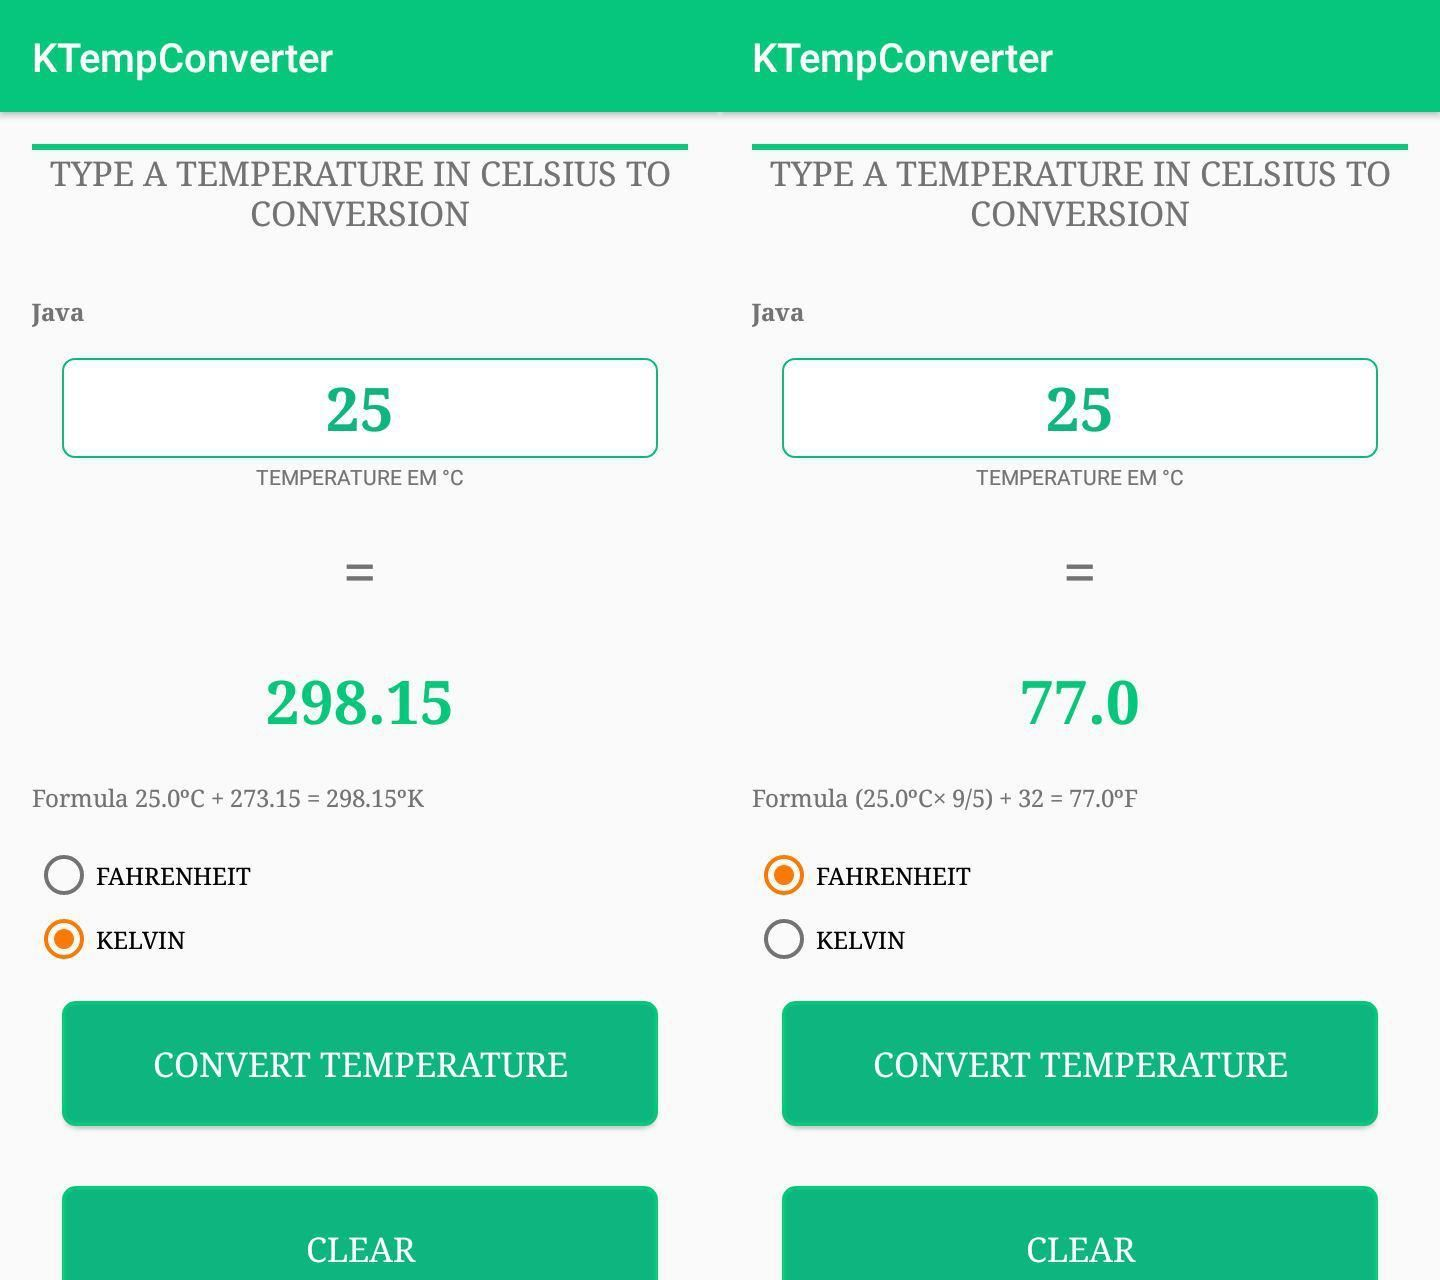
\includegraphics[scale=0.3]{imagens/java}
	\subcaption{\textbf{Fonte:} Elaborado pelo autor}
	\label{fig:figura3}
\end{figure*}
\FloatBarrier

As duas aplicações desempenham as mesmas funções e possuem os mesmos comportamentos, características e também o mesmo \textit{layout} (cores e disposição).  

\FloatBarrier
\begin{figure*}[!htbp]
	\centering
		\caption{Aplicação de Conversão de Medidas Termométricas escrito em \textit{Kotlin}}
	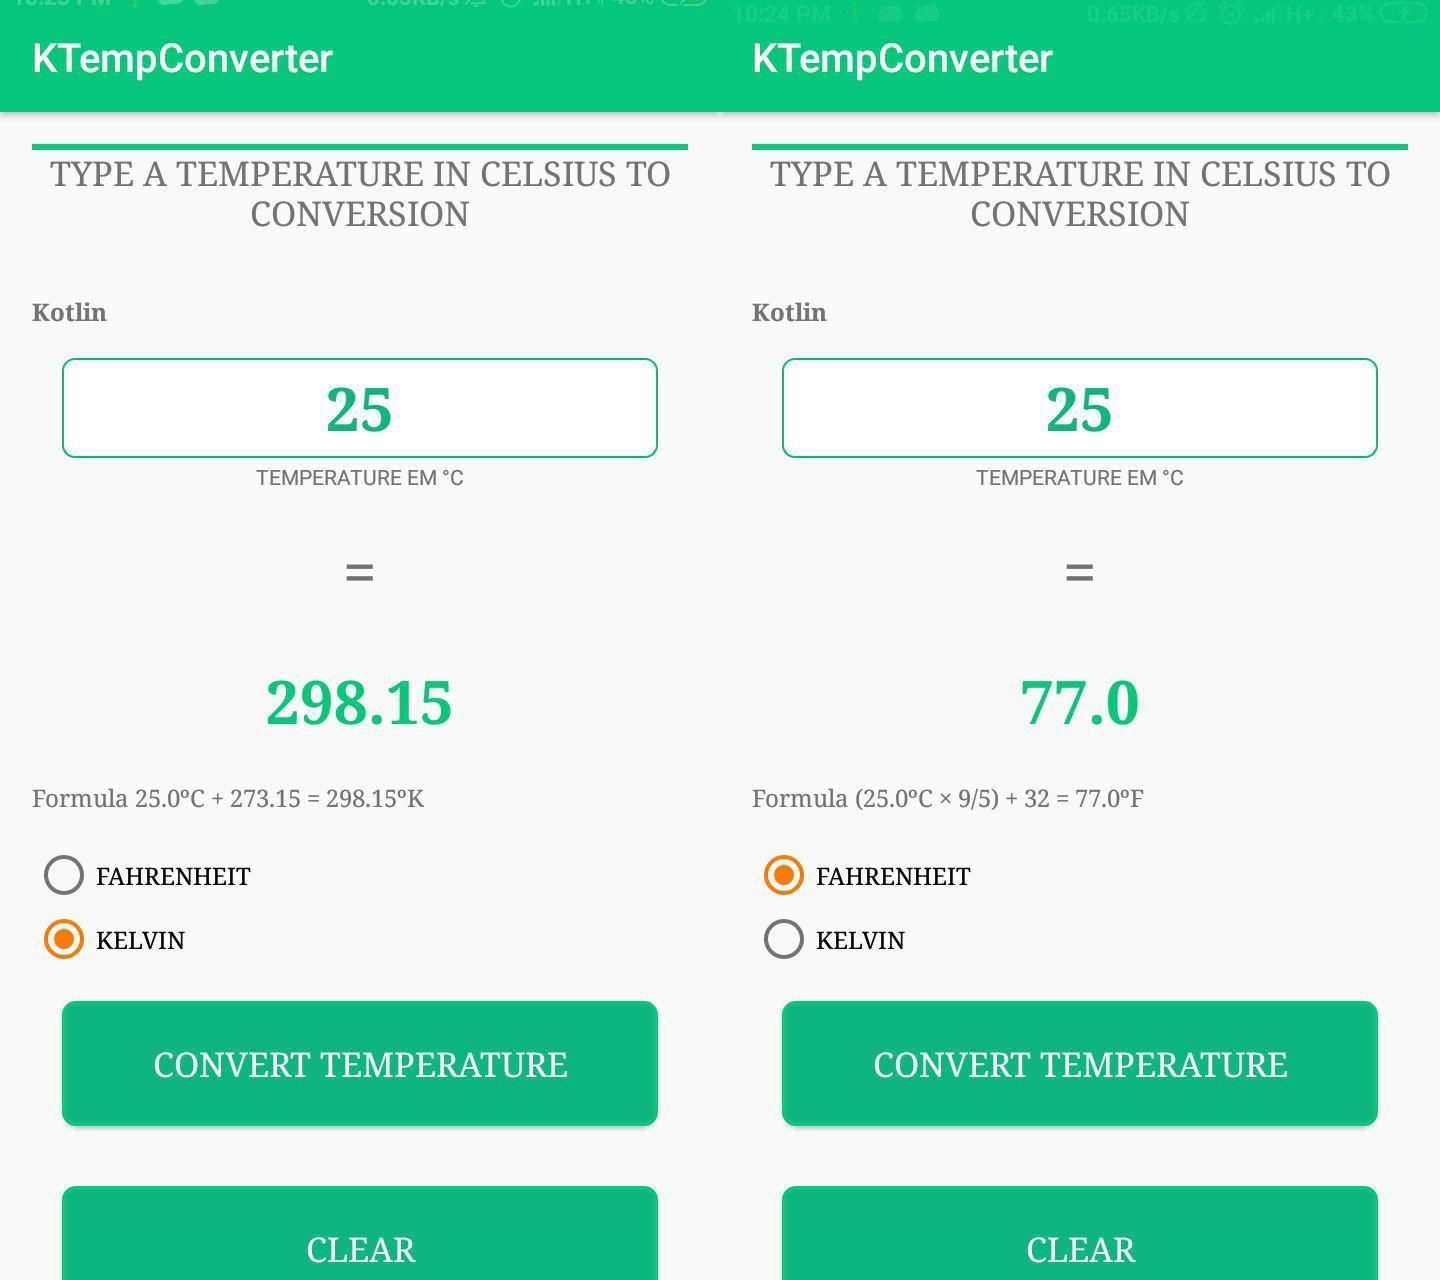
\includegraphics[scale=0.3]{imagens/kotlin}
	\subcaption{\textbf{Fonte:} Elaborado pelo autor}
	\label{fig:figura3}
\end{figure*}
\FloatBarrier

Tanto a aplicação \textit{Java} como a aplicação \textit{Kotlin} são capazes de realizar a conversão de uma medida em \textit{Celsius} inserida pelo usuário para \textit{Fahrenheit} ou \textit{Kelvin}.
\chapter{Resultados e Discussão}
\label{cap:04}

\section{Análise Qualitativa para Comparação entre \textit{Kotlin} e \textit{Java}}

Neste capítulo, apresenta-se análise a respeito do desempenho de cada uma das linguagens analisadas em âmbito geral, levando em consideração cada um dos experimentos em \textit{Kotlin} e \textit{Java}, desenvolvidos na seção anterior. 

\subsection{Comparação das Métricas}

Ao decorrer da presente seção, serão apresentados índices baseados no artigo: Análise Comparativa de Linguagens de Programação a partir de Problemas Clássicos da Computação, publico na revista Revista de Sistemas e Computação - RSC, desenvolvido na Universidade Federal de Itajubá do estado de Minas Gerais, no qual se estabelece um estudo comparativo sobre o tamanho dos algoritmos, velocidade de execução e tamanho em \textit{bytes} entre \textit{C}, \textit{Java} e \textit{Python}, ambas linguagens que encontram-se sempre no topo de pesquisas de popularidade. O estudo foi realizado por meio de experimentos matemáticos com diversas fórmulas amplamente conhecidas, os autores concluem com base nas comparações desenvolvidas, que a linguagem \textit{C} possui mais características para ser a escolhida.

Com o intuito de se estabelecer indicadores de qualidade, a fim de se efetuar uma avaliação referente aos algoritmos apresentados nos experimentos I, II, III, IV, V, VI e VII, foram definidos, como base, três índices qualificadores para avaliação, sendo eles:

\begin{itemize}
    \item Índice \textbf{A} (satisfatório): Implementação de algoritmo que realiza a utilização de poucos caracteres especiais, símbolos, assim como baixa quantidade de linhas de código;
     \item Índice \textbf{B} (parcialmente satisfatório): Implementação de algoritmo que se utiliza de mais caracteres especiais, símbolos ou maior quantidade de linhas de código;
      \item Índice \textbf{C} (insatisfatório): Implementação de algoritmo que se utiliza de maior quantidade de caracteres especiais, símbolos e linhas de código.
\end{itemize}

De acordo com os índices de qualidade exemplificados a seguir na Tabela 4, apresentam-se as métricas referentes aos códigos desempenhados no decorrer do capítulo 4:

\FloatBarrier
\begin{table}[!htbp]
\centering
\caption{Métrica Geral dos Experimentos}
	\begin{tabular}{ c | c | c }
		\hline
        \textbf{Métrica} &  \textbf{\textit{Kotlin}}    & \textbf{\textit{Java}}  \\ \hline
		
		  Caracteres utilizados   &     A 	       &            B     \\ \hline
		             
		  Linhas de código        &     A          &            B       \\ \hline
		             
		  Tamanho em \textit{bytes}        &     A          &            A      \\ \hline
		  
	\end{tabular}
	\\ \vspace{0.2cm}
	\textbf{Fonte:} Elaborada pelo autor
	\label{tab:exemplo}
\end{table}
\FloatBarrier

Conforme apresentado na Tabela 4, sobre a linguagem \textit{Kotlin} baseando-se unicamente nos algoritmos implementados e na formatação utilizada, facilita a menor utilização de caracteres especiais, símbolos e linhas de código, em comparação com a linguagem de programação \textit{Java}, recebendo assim, o índice de qualidade A em todos os quesitos analisados, levando em consideração os experimentos de introdução, sendo eles: I - \textit{Hello World}, II - operação aritmética de soma e III - classe \textit{Student}, também como os experimentos que demonstraram a implementação de aplicação de conversão de medidas termométricas, sendo eles:  IV - classe \textit{ThermometricScale}, V - interface \textit{Temperature}, VI - classe \textit{Adapter} e VII - classe \textit{Activity Main}.

\subsection{Pontos Positivos e Negativos da Adoção do Kotlin}

No ato de integrar-se em um projeto já existente, a compatibilidade com a linguagem de programação \textit{Kotlin}, observa-se um aumento de alguns segundos no tempo de execução da aplicação, e em caso de uma aplicação escrita somente em \textit{Kotlin}, o tempo de execução também é maior se comparada a uma aplicação desenvolvida em \textit{Java}. Por mais que seja possível literalmente misturar códigos em \textit{Java} e \textit{Kotlin} no mesmo projeto e até no mesmo arquivo, observa-se que para aproveitar-se todos os recursos oferecidos pela nova linguagem, como tornar o código mais enxuto e aumentar sua flexibilidade, necessita-se de consultas e estudos a documentação, uma vez que o recurso de conversão de \textit{Java} para \textit{Kotlin} que é disponibilizado nativamente pela \textit{IDE Android Studio} em versões mais recentes e por meio de \textit{plugins} em versões anteriores, não realiza a conversão da forma mais enxuta e direta possível, mas sim da forma mais verbosa, como por exemplo, a não utilização do recurso de importação de todos os \textit{widgets} utilizados no arquivo \textit{XML} de \textit{layout}, conforme demonstrado no experimento VII \textit{activity main}. 

O fato de \textit{Kotlin} ser totalmente integrada com a \textit{IDE Android Studio} torna a sua utilização/adoção bem atrativa e descomplicada. A compatibilidade da linguagem com \textit{Java} torna o desenvolvimento mais leve, deixando a cargo do desenvolvedor, escolher qual sintaxe, estilo e padronização de escrita de código utilizar, como por exemplo optar por utilizar ponto e vírgula ao final de cada instrução (\textit{Java}) ou não (\textit{Kotlin}). A curva de aprendizado apresenta-se baixa para desenvolvedores com conhecimento prévio em \textit{Java} e nas particularidades do desenvolvimento móvel voltado para o dispositivos móveis e o ecossistema da plataforma \textit{Android}.

\section{Análise Quantitativa para Comparação entre \textit{Kotlin} e \textit{Java}}

Para efetuar a comparação entre as linguagens \textit{Java} e \textit{Kotlin}, utiliza-se ferramenta disponibilizada de forma gratuita no endereço \textit{web} \url{https://www.4devs.com.br/analisar_textos}, que realiza a funcionalidade de contabilização de caracteres, palavras e de linhas de código. Conforme apresentado na Figura 13 a seguir, após inserir o algoritmo a ser analisado, logo abaixo do campo de texto, apresentam-se os campos onde são disponibilizados os valores.

\FloatBarrier
\begin{figure*}[!htbp]
	\centering
		\caption{Ferramenta de contagem de caracteres, palavras e linhas}
	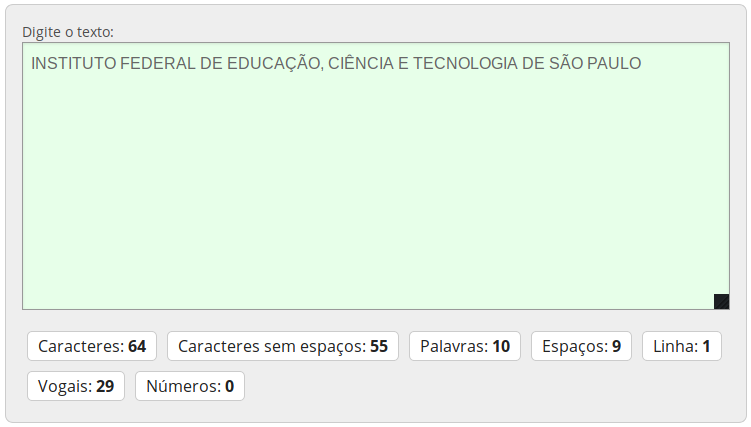
\includegraphics[scale=0.8]{imagens/4devs}
	\subcaption{\textbf{Fonte:} \url{https://www.4devs.com.br/analisar_textos}}
	\label{fig:figura3}
\end{figure*}
\FloatBarrier

Nas subseções posteriores, apresentam-se as tabelas com as devidas métricas de quantidade de caracteres, linhas de código e tamanho em \textit{bytes}, ambas as métricas obtidas por meio da disponibilização dos trechos de códigos utilizados nos experimentos, conforme demonstrado na Figura 13.

\subsection{Experimento I}

No exemplo de implementação de um simples e introdutório algoritmo de \textit{Hello World}, \textit{Kotlin} atingiu o objetivo, com uma menor quantidade de caracteres utilizados, linhas de código e consequentemente de \textit{bytes}, conforme Tabela 5 a seguir.

\FloatBarrier
\begin{table}[!htbp]
\centering
\caption{Métricas \textit{Hello World}}
	\begin{tabular}{ c | c | c }
		\hline
           \textbf{Métrica} &            \textbf{\textit{Kotlin}}    & \textbf{\textit{Java}}  \\ \hline
		
		  Caracteres utilizados   &     39 	           &             116     \\ \hline
		             
		  Linhas de código        &     03             &             05       \\ \hline
		             
		  Tamanho em \textit{bytes}        &     39             &             117      \\ \hline
		  
	\end{tabular}
	\\ \vspace{0.2cm}
	\textbf{Fonte:} Elaborada pelo autor
	\label{tab:exemplo}
\end{table}
\FloatBarrier

\subsection{Experimento II}

De acordo com a Tabela 6, no experimento de implementação de operação de soma, que retorna a soma de dois valores fixos e inteiros, interpolados com um pequeno trecho de texto, \textit{Kotlin} obteve os menores índices em todas as métricas analisadas.


\FloatBarrier
\begin{table}[!htbp]
\centering
\caption{Métricas Operação Aritmética de Soma}
	\begin{tabular}{ c | c | c }
		\hline
          \textbf{Métrica} &          \textbf{\textit{Kotlin}}    & \textbf{\textit{Java}}  \\ \hline
		
		  Caracteres utilizados   &     81 	           &            159      \\ \hline
		             
		  Linhas de código        &     5             &            6      \\ \hline
		             
		  Tamanho em \textit{bytes}        &     80             &           159      \\ \hline
		  
	\end{tabular}
	\\ \vspace{0.2cm}
	\textbf{Fonte:} Elaborada pelo autor
	\label{tab:exemplo}
\end{table}
\FloatBarrier

\subsection{Experimento III}

No experimento de implementação de uma classe que abstrai de maneira simples, as características de um estudante, \textit{Kotlin} demonstra a possibilidade de evitar códigos desnecessários em algoritmos comumente utilizados, possibilitando a economia de mais de mil caracteres e 60 linhas de implementação, conforme Tabela 7. 

\FloatBarrier
\begin{table}[!htbp]
\centering
\caption{Métricas Classe \textit{Student}}
	\begin{tabular}{ c | c | c }
		\hline
          \textbf{Métrica} &          \textbf{\textit{Kotlin}}    & \textbf{\textit{Java}}  \\ \hline
		
		  Caracteres utilizados   &     163 	      &          1.607      \\ \hline
		             
		  Linhas de código        &     4             &            67      \\ \hline
		             
		  Tamanho em \textit{bytes}        &     163           &          1.600     \\ \hline
		  
	\end{tabular}
	\\ \vspace{0.2cm}
	\textbf{Fonte:} Elaborada pelo autor
	\label{tab:exemplo}
\end{table}
\FloatBarrier

\subsection{Experimento IV}

Com a implementação da classe \textit{ThermometricScale}, de acordo com a Tabela 8, observa-se por meio da implementação da declaração de funções, parâmetros e seus respectivos retornos disponível em \textit{Kotlin}, economiza-se diversas linhas de código, podendo variar de acordo com a abordagem do(s) desenvolvedor(s).

\FloatBarrier
\begin{table}[!htbp]
\centering
\caption{Métricas Classe \textit{ThermometricScale}}
	\begin{tabular}{ c | c | c }
		\hline
          \textbf{Métrica} &          \textbf{\textit{Kotlin}}    & \textbf{\textit{Java}}  \\ \hline
		
		  Caracteres utilizados   &     283 	      &          363      \\ \hline
		             
		  Linhas de código        &     9             &           16      \\ \hline
		             
		  Tamanho em \textit{bytes}        &     285           &          364      \\ \hline
		  
	\end{tabular}
	\\ \vspace{0.2cm}
	\textbf{Fonte:} Elaborada pelo autor
	\label{tab:exemplo}
\end{table}
\FloatBarrier

\subsection{Experimento V}

No experimento no qual implementa-se a função da interface \textit{Temperature} a ser implementada, \textit{Kotlin} e \textit{Java} utilizam a mesma quantidade de linhas de código, \textit{Kotlin} obtém os resultados menores na métrica de caracteres utilizados e tamanho em \textit{bytes}, conforme Tabela 9.

\FloatBarrier
\begin{table}[!htbp]
\centering
\caption{Métricas Interface \textit{Temperature}}
	\begin{tabular}{ c | c | c }
		\hline
          \textbf{Métrica} &         \textbf{\textit{Kotlin}}    & \textbf{\textit{Java}}  \\ \hline
		
		  Caracteres utilizados   &     143 	      &          155      \\ \hline
		             
		  Linhas de código        &     5             &           5      \\ \hline
		             
		  Tamanho em \textit{bytes}        &     144           &          156      \\ \hline
		  
	\end{tabular}
	\\ \vspace{0.2cm}
	\textbf{Fonte:} Elaborada pelo autor
	\label{tab:exemplo}
\end{table}
\FloatBarrier

\subsection{Experimento VI}

De acordo com a Tabela 10, na implementação da classe que tem por objetivo ser um adaptador no aplicativo de conversão, demonstra-se que Java necessita de maiores quantidades de linhas de código, caracteres e um tamanho superior em \textit{bytes}.

\FloatBarrier
\begin{table}[!htbp]
\centering
\caption{Métricas Classe \textit{Adapter}}
	\begin{tabular}{ c | c | c }
		\hline
            \textbf{Métrica} &         \textbf{\textit{Kotlin}}    & \textbf{\textit{Java}}  \\ \hline
		
		  Caracteres utilizados   &     605 	      &          741      \\ \hline
		             
		  Linhas de código        &     19            &           26      \\ \hline
		             
		  Tamanho em \textit{bytes}        &     608           &          742      \\ \hline
		  
	\end{tabular}
	\\ \vspace{0.2cm}
	\textbf{Fonte:} Elaborada pelo autor
	\label{tab:exemplo}
\end{table}
\FloatBarrier

\subsection{Experimento VII}

Na classe principal do programa de conversão de Celsius para Fahrenheit e Kelvin, de acordo com a implementação utilizada, \textit{Java} demonstra a necessidade da utilização de mais caracteres, aumentando a quantidade de linhas de código , consequentemente, o tamanho em \textit{bytes}, conforme Tabela 11.

\FloatBarrier
\begin{table}[!htbp]
\centering
\caption{Métricas Classe \textit{Activity Main}}
	\begin{tabular}{ c | c | c }
		\hline
            \textbf{Métrica} &        \textbf{\textit{Kotlin}}    & \textbf{\textit{Java}}  \\ \hline
		
		  Caracteres utilizados   &     2.404 	      &          3.179      \\ \hline
		             
		  Linhas de código        &     74            &           93      \\ \hline
		             
		  Tamanho em \textit{bytes}        &     3.200           &          3.800      \\ \hline
		  
	\end{tabular}
	\\ \vspace{0.2cm}
	\textbf{Fonte:} Elaborada pelo autor
	\label{tab:exemplo}
\end{table}
\FloatBarrier
\chapter{Conclusões}
\label{cap:05}

Este trabalho abordou um estudo analítico entre tecnologias diferentes, mas que servem a um mesmo propósito, e um estudo de usabilidade sobre a linguagem de programação \textit{Kotlin}, referente à todo o ecossistema que envolve a plataforma \textit{Android}.

Adicionalmente, foram apresentados, em caráter introdutório, as principais tecnologias que fazem parte do desenvolvimento voltado para os dispositivos móveis, desde os meios para a elaboração de aplicações tanto nativas e específicas para apenas uma plataforma, como aplicações que atingem ambos os públicos com tecnologias denominadas híbridas/multiplataforma. Também foram apresentados os conceitos de qualidade de código por meio de ferramentas e da reescrita, e detalharam-se alguns trabalhos com segmento semelhante ao contexto deste trabalho.

Baseando-se em três índices qualificadores de código, sendo eles, a quantidade de caracteres, as linhas de código utilizadas e o tamanho do arquivo em \textit{bytes}, foram implementados 07 experimentos práticos, desde alguns algoritmos mais simples como operação matemática, \textit{Hello World} e classe \textit{model}, finalizando com uma aplicação móvel \textit{Android} que realiza a conversão de medidas termométricas de Celsius para Fahrenheit e/ou Kelvin, por meio da interação com o usuário, baseada um padrão de projeto. De acordo com os códigos desempenhados foi realizada a comparação entre a linguagem \textit{Kotlin} e \textit{Java}, no qual, \textit{Kotlin} mostrou-se, tão eficaz quanto Java, chegando ao mesmo resultado, com menor necessidade de caracteres, linhas de código e da mesma forma tamanho final em \textit{bytes}, sendo superior em todos os experimentos implementados.

Somando-se todos os trechos de código demonstrados nos experimentos, em \textit{Java} foram necessários: \textbf{6.320} caracteres, \textbf{218} linhas de código e \textbf{6.938} bytes. Por outro lado, com \textit{Kotlin}, obteve-se os mesmos resultados finais, por meio de: \textbf{3.718} caracteres, \textbf{119} linhas de código e \textbf{4.480} bytes.
%\begin{itemize}
    %\\item \textbf{6.320} caracteres;
    %\\item\textbf{218} linhas de código;
    %\\item  \textbf{6.938} bytes.
%\\end{itemize}

 %\Toda via, com o \textit{Kotlin}, obteve-se os mesmos %\resultados finais, por meio de:
%\ \begin{itemize}
 %\\item  \textbf{3.718} caracteres;
 %\ \item \textbf{119} linhas de código;
 %\ \item \textbf{4.480} bytes.
 %\\end{itemize}
Foram apresentados os pontos negativos e positivos na adoção da tecnologia \textit{Kotlin} como linguagem de programação, onde destacou-se como negativo o aumento no tempo de execução de projetos \textit{Kotlin} e como positivo, a sua fácil adaptação para programadores com conhecimento prévio.

Para trabalhos futuros, o conceito da diminuição de utilização de códigos desnecessários no desenvolvimento de \textit{software} apresentados neste trabalho pode motivar novas pesquisas relacionadas, como a comparação de tecnologias que propõe-se a entregar aplicações móveis multiplataforma e nativas, ou seja, para \textit{Android} e \textit{iOS}. As tecnologias e linguagens adotadas e desenvolvidas por grandes empresas que são referência no meio tecnológico, como a ferramenta \textit{Flutter} que utiliza a linguagem \textit{Dart} ambos projetos criados pela \textit{Google} e o \textit{framework} \textit{React Native} criado pelo \textit{Facebook} que utiliza \textit{JavaScript} são exemplos de alternativas emergentes no momento em que esse trabalho foi realizado. Outra opção de futuros projetos relacionados a este trabalho de conclusão de curso seria uma nova comparação entre as linguagens \textit{Java} e \textit{Kotlin}, mas com foco em \textit{CRUD's}\footnote[1]{Acrônimo em inglês para operações básicas de um sistema, sendo elas: C de  \textit{create} (inclusão), R de  \textit{read} (leitura), U de  \textit{update} (atualização) e D de  \textit{delete} (remoção) \cite{CRUD}}, desenvolvimento da Sequência de \textit{Fibonacci},  operações matemáticas e cálculos mais elaborados e de algoritmos de encriptação para se medir a complexidade em cada uma das abordagens.





\input{capitulo06Cronograma}






% ---------------------------------------------------------------------------------
%                                 ELEMENTOS PÓS-TEXTUAIS
% ---------------------------------------------------------------------------------
\postextual


% ----------------------------------------------------------
% Referências bibliográficas
% ----------------------------------------------------------
\bibliography{referencias}


% ----------------------------------------------------------
% Glossário
% ----------------------------------------------------------
%
% Consulte o manual da classe abntex2 para orientações sobre o glossário.
%
%\glossary


% ----------------------------------------------------------
% Apêndices
% ----------------------------------------------------------
% % Texto ou documento elaborado pelo autor, a fim de complementar sua argumentação, sem prejuízo da unidade nuclear do trabalho.

% ---
% Inicia os apêndices
% ---
\begin{apendicesenv}
	
	% Imprime uma página indicando o início dos apêndices
	\partapendices
	
	% ----------------------------------------------------------
	\chapter{Título do Apêndice A}
	% ----------------------------------------------------------
	
	Texto do Apêndice A.
	
	
	
	% ----------------------------------------------------------
	\chapter{Título do Apêndice B}
	% ----------------------------------------------------------
	
	Texto do Apêndice B.
	
	
	
	% ----------------------------------------------------------
	\chapter{Título do Apêndice C}
	% ----------------------------------------------------------
	
	Texto do Apêndice C.
	
	
	
	% ----------------------------------------------------------
	\chapter{Título do Apêndice D}
	% ----------------------------------------------------------
	
	Texto do Apêndice D.
	
	
	
	% ----------------------------------------------------------
	\chapter{Título do Apêndice E}
	% ----------------------------------------------------------
	
	Texto do Apêndice E.
	
	
	
\end{apendicesenv}
% ---


% ----------------------------------------------------------
% Anexos
% ----------------------------------------------------------
% % Texto ou documento não elaborado pelo autor, que serve de fundamentação, comprovação e ilustração.

% ---
% Inicia os anexos
% ---
\begin{anexosenv}
	
	% Imprime uma página indicando o início dos anexos
	\partanexos
	
	% ----------------------------------------------------------
	\chapter{Título do Anexo A}
	% ----------------------------------------------------------
	
	Texto do Anexo A.
	
	
	
	% ----------------------------------------------------------
	\chapter{Título do Anexo B}
	% ----------------------------------------------------------
	
	Texto do Anexo B.
	
	
	
	% ----------------------------------------------------------
	\chapter{Título do Anexo C}
	% ----------------------------------------------------------
	
	Texto do Anexo C.
	
	
	
	% ----------------------------------------------------------
	\chapter{Título do Anexo D}
	% ----------------------------------------------------------
	
	Texto do Anexo D.
	
	
	
	% ----------------------------------------------------------
	\chapter{Título do Anexo E}
	% ----------------------------------------------------------
	
	Texto do Anexo E.
	
	
	
\end{anexosenv}


%---------------------------------------------------------------------
% ÍNDICE REMISSIVO
%---------------------------------------------------------------------

%\phantompart

%\printindex


\end{document}
